% !TeX encoding = UTF-8
% !TeX program = xelatex
% !TeX spellcheck = en_US

\documentclass[degree=master]{thuthesis}
  % 学位 degree:
  %   doctor | master | bachelor | postdoc
  % 学位类型 degree-type:
  %   academic(默认)| professional


% 论文基本配置,加载宏包等全局配置
% !TeX root = ../main.tex

% 论文基本信息配置

\thusetup{
  %******************************
  % 注意:
  %   1. 配置里面不要出现空行
  %   2. 不需要的配置信息可以删除
  %******************************
  %
  % 标题
  %   可使用“\\”命令手动控制换行
  %
  title  = {清华大学学位论文 \LaTeX{} 模板\\使用示例文档 v\version},
  title* = {An Introduction to \LaTeX{} Thesis Template of Tsinghua
            University v\version},
  %
  % 学位
  %   1. 学术型
  %      - 中文
  %        需注明所属的学科门类,例如:
  %        哲学、经济学、法学、教育学、文学、历史学、理学、工学、农学、医学、
  %        军事学、管理学、艺术学
  %      - 英文
  %        博士:Doctor of Philosophy
  %        硕士:
  %          哲学、文学、历史学、法学、教育学、艺术学门类,公共管理学科
  %          填写“Master of Arts“,其它填写“Master of Science”
  %   2. 专业型
  %      直接填写专业学位的名称,例如:
  %      教育博士、工程硕士等
  %      Doctor of Education, Master of Engineering
  %   3. 本科生不需要填写
  %
  degree-name  = {工学学士},
  degree-name* = {Bachelor of Science},
  %
  % 培养单位
  %   填写所属院系的全名
  %
  department = {计算机科学与技术系},
  %
  % 学科
  %   1. 学术型学位
  %      获得一级学科授权的学科填写一级学科名称,其他填写二级学科名称
  %   2. 工程硕士
  %      工程领域名称
  %   3. 其他专业型学位
  %      不填写此项
  %   4. 本科生不需要填写
  %
  discipline  = {计算机科学与技术},
  discipline* = {Computer Science and Technology},
  %
  % 姓名
  %
  author  = {霍江浩},
  author* = {Huo Jianghao},
  %
  % 指导教师
  %   中文姓名和职称之间以英文逗号“,”分开,下同
  %
  supervisor  = {方斌},
  supervisor* = {Fang Bin},
  %
  % 联合指导教师
  %
  % joint-supervisor  = {某某某教授},
  % joint-supervisor* = {Professor Mou Moumou},
  %
  % 日期
  %   使用 ISO 格式;默认为当前时间
  %
  % date = {2019-07-07},
  %
  % 密级和年限
  %   秘密, 机密, 绝密
  %
  % secret-level = {秘密},
  % secret-year  = {10},
  %
  % 博士后专有部分
  %
  % clc                = {分类号},
  % udc                = {UDC},
  % id                 = {编号},
  % discipline-level-1 = {计算机科学与技术},  % 流动站(一级学科)名称
  % discipline-level-2 = {系统结构},          % 专业(二级学科)名称
  % start-date         = {2011-07-01},        % 研究工作起始时间
}

%% Put any packages you would like to use here

% 表格中支持跨行
\usepackage{multirow}

% 跨页表格
\usepackage{longtable}

% 固定宽度的表格
\usepackage{tabularx}

% 表格中的反斜线
\usepackage{diagbox}

% 确定浮动对象的位置,可以使用 H,强制将浮动对象放到这里(可能效果很差)
\usepackage{float}

% 浮动图形控制宏包。
% 允许上一个 section 的浮动图形出现在下一个 section 的开始部分
% 该宏包提供处理浮动对象的 \FloatBarrier 命令,使所有未处
% 理的浮动图形立即被处理。这三个宏包仅供参考,未必使用:
% \usepackage[below]{placeins}
% \usepackage{floatflt} % 图文混排用宏包
% \usepackage{rotating} % 图形和表格的控制旋转

% 定理类环境宏包
\usepackage[amsmath,thmmarks,hyperref]{ntheorem}

% 给自定义的宏后面自动加空白
% \usepackage{xspace}

% 借用 ltxdoc 里面的几个命令。
\def\cmd#1{\cs{\expandafter\cmd@to@cs\string#1}}
\def\cmd@to@cs#1#2{\char\number`#2\relax}
\DeclareRobustCommand\cs[1]{\texttt{\char`\\#1}}

\newcommand*{\meta}[1]{{%
  \ensuremath{\langle}\rmfamily\itshape#1\/\ensuremath{\rangle}}}
\providecommand\marg[1]{%
  {\ttfamily\char`\{}\meta{#1}{\ttfamily\char`\}}}
\providecommand\oarg[1]{%
  {\ttfamily[}\meta{#1}{\ttfamily]}}
\providecommand\parg[1]{%
  {\ttfamily(}\meta{#1}{\ttfamily)}}
\providecommand\pkg[1]{{\sffamily#1}}

% 定义所有的图片文件在 figures 子目录下
\graphicspath{{figures/}}

% 数学命令
\input{math_commands.tex}

% 定义自己常用的东西
% \def\myname{薛瑞尼}

% hyperref 宏包在最后调用
\usepackage{hyperref}



\begin{document}

% 封面
\maketitle

% 使用授权的说明
\copyrightpage

\frontmatter
% !TeX root = ../main.tex

% 中英文摘要和关键字

\begin{abstract}

  本文总结了目前机器人学习领域的研究现状,以及主要数据集。并且设计、发布了多机器人
  学习数据集THUR-20。在完成THUR-20的设计、采集之后,作者使用机器人学习领域经常
  使用的Behavior Cloning方法验证了THUR-20的可用性,实验表明,本文发布的THUR-20
  数据集在有效性和易用性上有优越的表现。

  本文的创新点主要有
  \begin{itemize}
    \item 全面的总结了机器人学习领域的现状及现有数据集的优缺点;
    \item 设计发布了THUR-20数据集的标准和采集方案;
    \item 完成了THUR-20初始数据的采集;
    \item 使用Behavior Cloning方法验证了THUR-20的可用性;
  \end{itemize}

  % 关键词用“英文逗号”分隔
  \thusetup{
    keywords = {Robotics Learning, Dataset, Behavior Cloning, THUR-20},
  }
\end{abstract}

\begin{abstract*}

  A log of BLALBALBA...

  \thusetup{
    keywords* = {Robotics Learning, Dataset, Behavior Cloning, THUR-20},
  }
\end{abstract*}


% 目录
\tableofcontents

% 符号对照表
%\input{data/denotation}


% 正文部分
\mainmatter
% !TeX root = ../main.tex

\chapter{移动操作机器人的国内外现状}
\label{cha:intro}

\section{移动操作机器人概念}
\label{cha:base_comcept}

移动操作机器人(Mobile Manipulator)目前仍然是一个非常宽泛的概念,通常我们认为,典型的移动操作
机器人是由一台机械臂和一个可自由移动的平台组成的,机械臂通过某种方式挂载在平台上\cite{bostelman2016survey}。
近年来,随着科技的飞速发展以及制造业转型的巨大压力,移动操作机器人成为新的研究热点,在学术界及
工业界受到了广泛关注\cite{schneier2015literature}。移动操作机器人已经被广泛的应用到了航天\cite{ambrose2004mobile}、医药、制造\cite{guizzo2011meka}、清洁、服务等多个场景,
在各个领域发挥着重要的作用。但移动操作机器人在性能和功能上还远远没有达到我们期待的水平,相
关研究及工业尝试还需要很长时间的发展。

广义的移动操作机器人除机械臂外,可依赖的平台非常多样,除了常见的轮式底盘、平衡车式底盘外,还可
使用无人机作为移动平台,甚至仿人的双足行走底盘。无人机平台的移动操作机器人有夹爪式、机械臂式等
各种种类,近年来也广泛的
受到各界的关注\cite{ruggiero2018aerial}。相比于无人机或者足式底盘,轮式底盘的移动操作机器人负载更
高,性能更强劲,应用更加广泛,功能更加多样,品种也更加丰富,因此本文主要论述以轮式底盘作为移动
平台的移动操作机器人,并给出相应的控制方法。

\section{移动操作机器人国内外应用现状}
\label{cha:application}

近年来,国内外机器人相关的创业公司层出不穷,移动操作机器人行业也是投资机构聚焦的热点。下面本文
将分别介绍移动操作机器人的两大主要部分:机械臂以及移动底盘的应用历史与现状,随后介绍移动操作机器人
作为整体的应用情况。

机械臂作为主要生产工具在制造业承担作用的历史非常久,机械臂在制造业最早的规模化应用被认为诞生
在汽车制造领域。同其他行业相比,汽车领域产品款式固定,出货量大,规模效应强,这些特性使得基于硬编码
控制的大型高精度机械臂得到广泛应用,如图~\ref{fig:armcar} 展示了工业机械臂在汽车产线上应用
的场景。以汽车工业为代表的自动化机器人应用大部分为高精度工业机械臂,其发展已经有近
半个世纪的历史,自1973年ABB和KUKA将工业机器人推向市场后,这一行业迎来了飞速发展,工业机械臂
的厂商不断增加,款式与性能持续丰富,各种面对细分领域的工业机械臂相继面世,如图~\ref{fig:industry_arms}。

\begin{figure}
\centering
\begin{subfigure}{1.\textwidth}
  \centering
  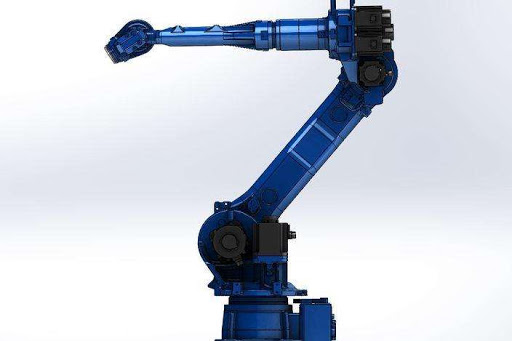
\includegraphics[height=3.5cm]{arm1.jpg}
  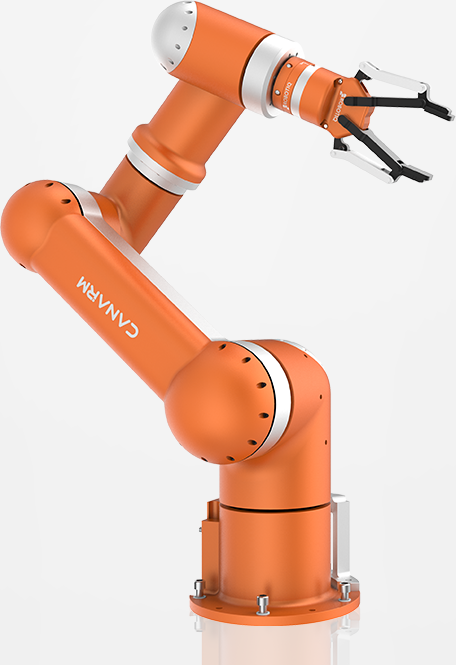
\includegraphics[height=3.5cm]{arm2.png}
  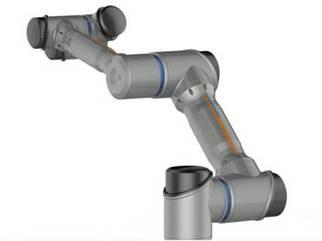
\includegraphics[height=3.5cm]{arm4.jpg}\\
  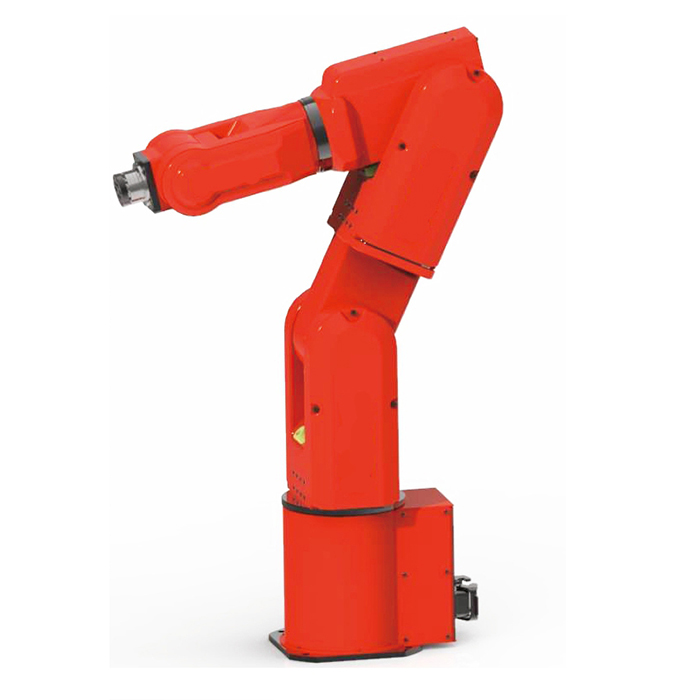
\includegraphics[height=3.5cm]{arm3.jpg}
  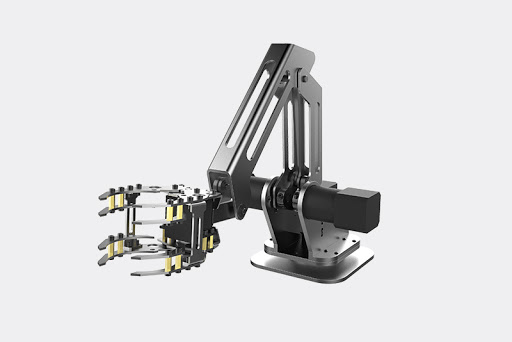
\includegraphics[height=3.5cm]{arm5.jpg}
  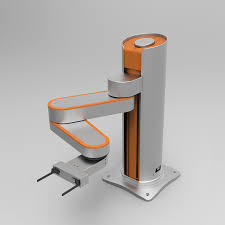
\includegraphics[height=3.5cm]{arm6.jpeg}
\end{subfigure}%
\caption{各式工业机械臂产品}
\label{fig:industry_arms}
\end{figure}


目前,国际
工业机器人领域有四大标杆企业,分别是瑞典 ABB、德国 KUKA、日本FANUC 和日本安川电机。四大厂商
各有所长,ABB擅长控制系统,KUKA优势在于系统集成应用与本体制造,FANUC长于数控系统,安川电机
的优势在于伺服电机制造和运动控制器的研发。除四大头部企业外,美国 Adept Technology、瑞士
Staubli、意大利Comau、日本的川崎、爱普生、那智不二越和中国新松机器人自动化股份有限公司也是
国际工业机器人的重要供应商\cite{huangxihuanReview}。

除汽车工业外,高精度工业机械臂在医疗
领域也取得了不俗的成绩,Intuitive Surgical公司研发的“达芬奇”手术机器人在世界范围内广泛应用,
我国于2006年引入第一套达芬奇手术系统,至今各式手术机器人在中国已累计完成10万例外科手术,如
图~\ref{fig:davinci}。我国华大智造研发的远程
超声检测系统~\ref{fig:huada},该系统在新冠疫情期间的武汉方舱医院内进行了应用测试\cite{wushengzheng20205g},取得了可喜的进展。


\begin{figure}
\centering
\begin{subfigure}{.5\textwidth}
  \centering
  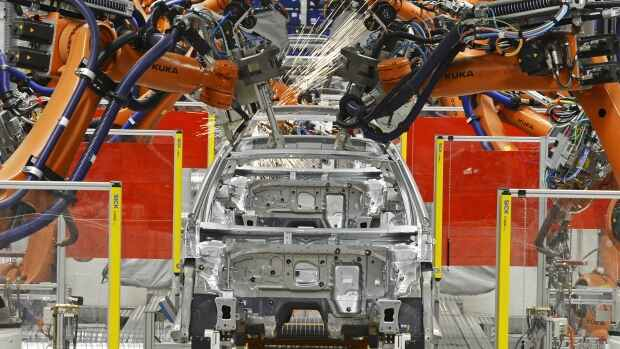
\includegraphics[height=3cm]{kuka_car.jpg}
  \caption{完全由库卡机械臂组成的汽车焊接流水线}
\end{subfigure}%
\begin{subfigure}{.5\textwidth}
  \centering
  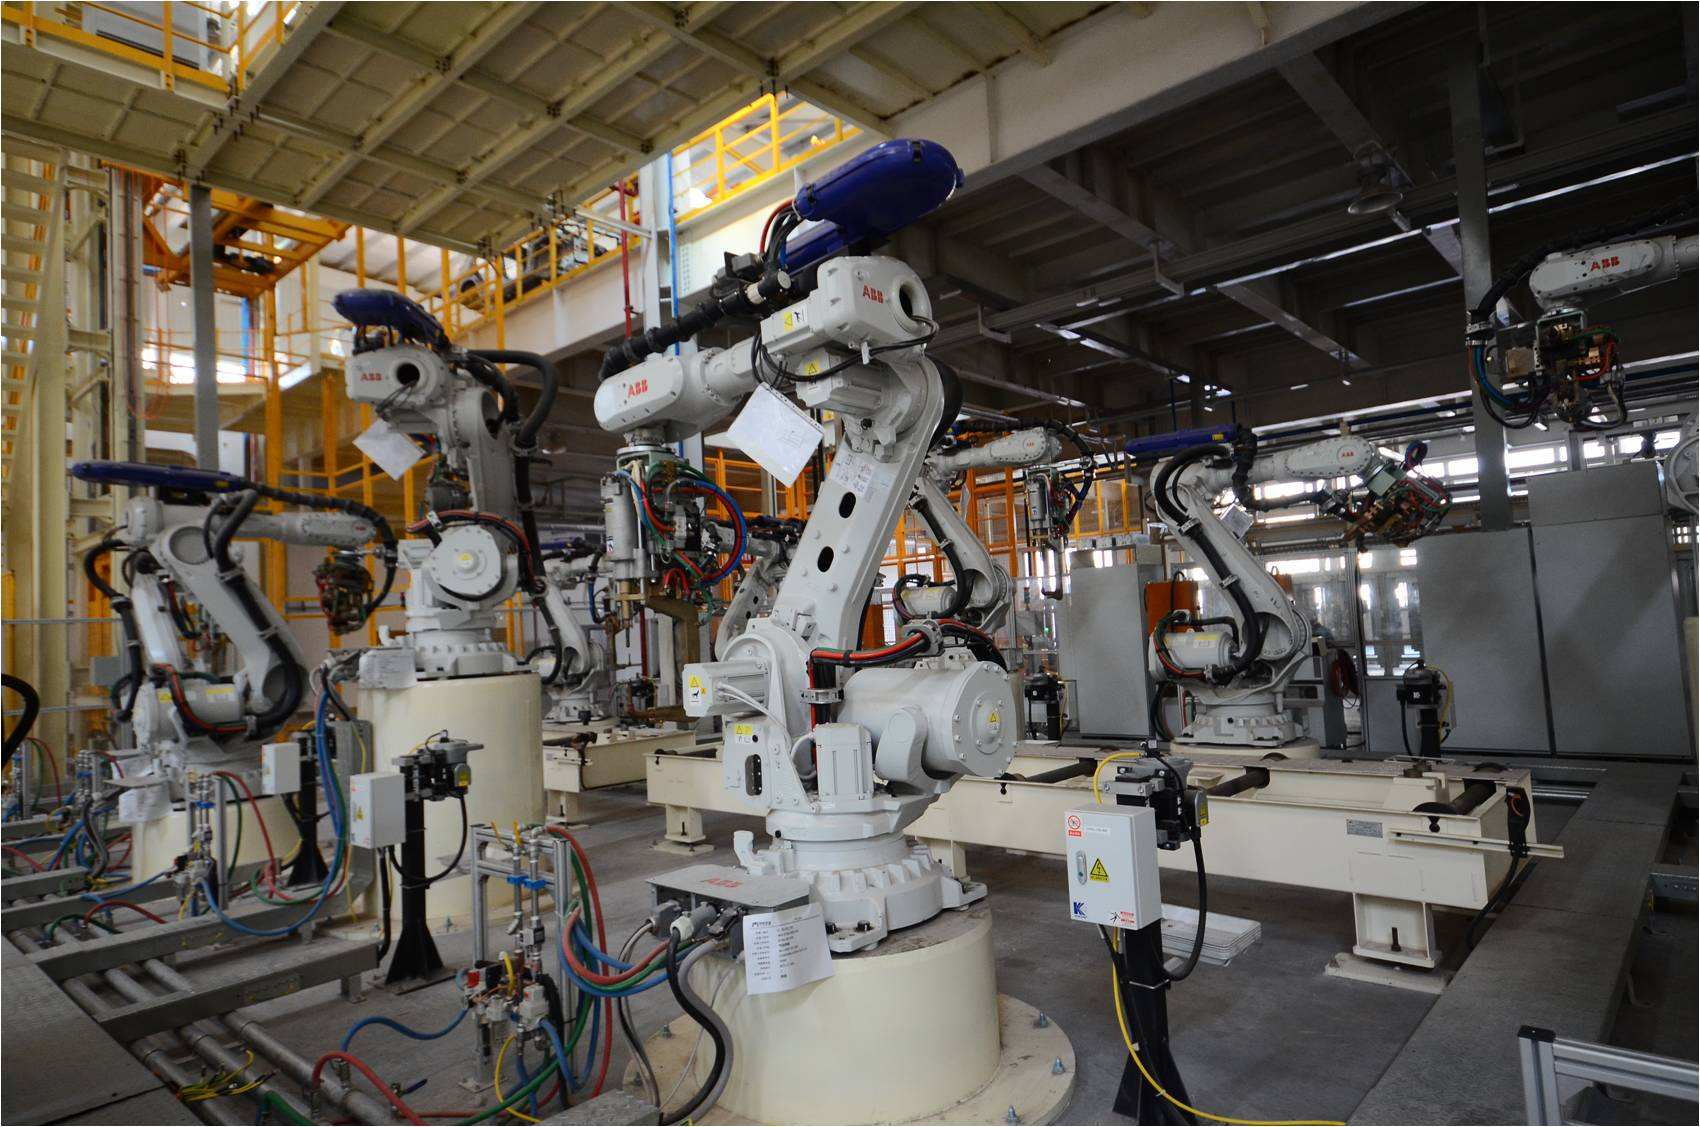
\includegraphics[height=3cm]{abb_car.jpeg}
  \caption{ABB机械臂组成的汽车零件装配产线}
\end{subfigure}
\caption{工业机械臂在流水线上工作}
\label{fig:armcar}
\end{figure}

\begin{figure}
\centering
\begin{subfigure}{.5\textwidth}
  \centering
  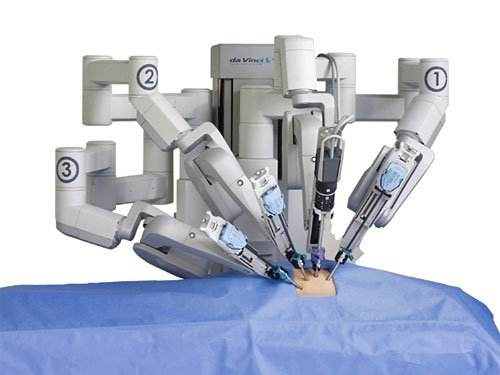
\includegraphics[height=4cm]{davinci.jpeg}
  \caption{达芬奇机器人在工作}
  \label{fig:davinci}
\end{subfigure}%
\begin{subfigure}{.5\textwidth}
  \centering
  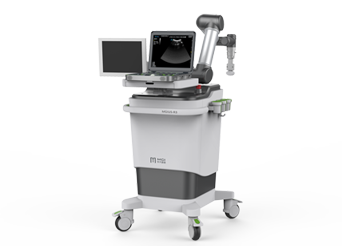
\includegraphics[height=4cm]{huada.png}
  \caption{华大智造的远程超声检测机器人}
  \label{fig:huada}
\end{subfigure}%
\caption{机械臂产品在国内外医疗领域的应用}
\end{figure}



\iffalse % 删掉这些华而不实的玩意儿
    近年来,一些富有展示性的机械臂应用开始逐步面世,例如机器人调酒应用。
    最早引起轰动的是皇家加勒比游轮有限公司在其的最新款邮轮海洋量子号上的“仿生酒吧”中应用了机器人
    调酒师,如图~\ref{fig:liangzi_arm},很快各种调酒机器人被竞相开发出来,如意大利的机器人
    酒吧\ref{fig:italy_arm},拉斯维加斯的机器人调酒师\ref{fig:las_arm},以及我国哈工大开发的
    机器人调酒师\ref{fig:hgd_arm}。尽管机器人调酒目前并不能带来成本或者质量
    上的提升,但是机器人调酒的概念本身富有科技感,新鲜有趣充满噱头,是吸引消费者的一大亮点。


    \begin{figure}
    \centering
    \begin{subfigure}{.5\textwidth}
      \centering
      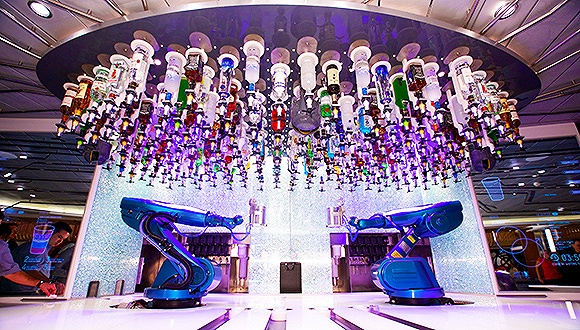
\includegraphics[height=3.5cm]{liangzi_arm.jpg}
      \caption{皇家加勒比海洋量子号的仿生酒吧}
      \label{fig:liangzi_arm}
    \end{subfigure}%
    \begin{subfigure}{.5\textwidth}
      \centering
      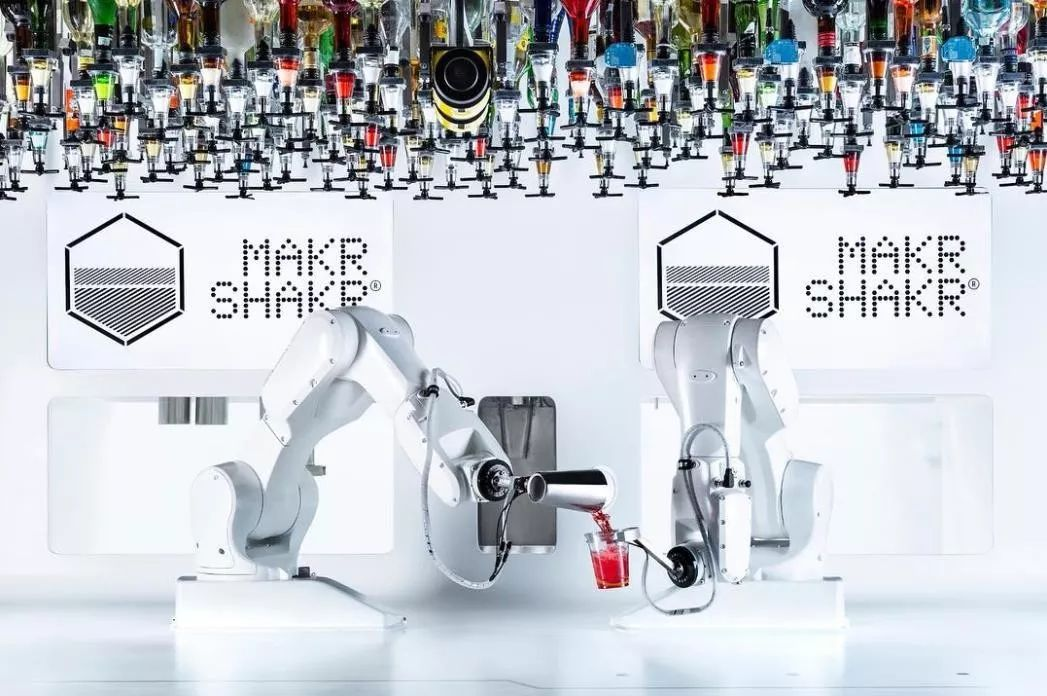
\includegraphics[height=3.5cm]{italy_arm.jpg}
      \caption{意大利The View机器人酒吧}
      \label{fig:italy_arm}
    \end{subfigure}%
    \\
    \begin{subfigure}{.5\textwidth}
      \centering
      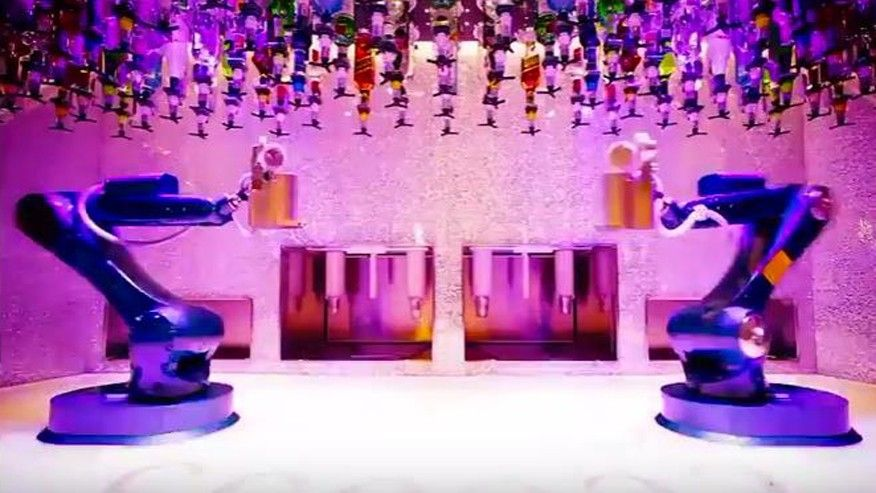
\includegraphics[height=3.5cm]{las_arm.jpg}
      \caption{拉斯维加斯微醺机器人酒吧}
      \label{fig:las_arm}
    \end{subfigure}%
    \begin{subfigure}{.5\textwidth}
      \centering
      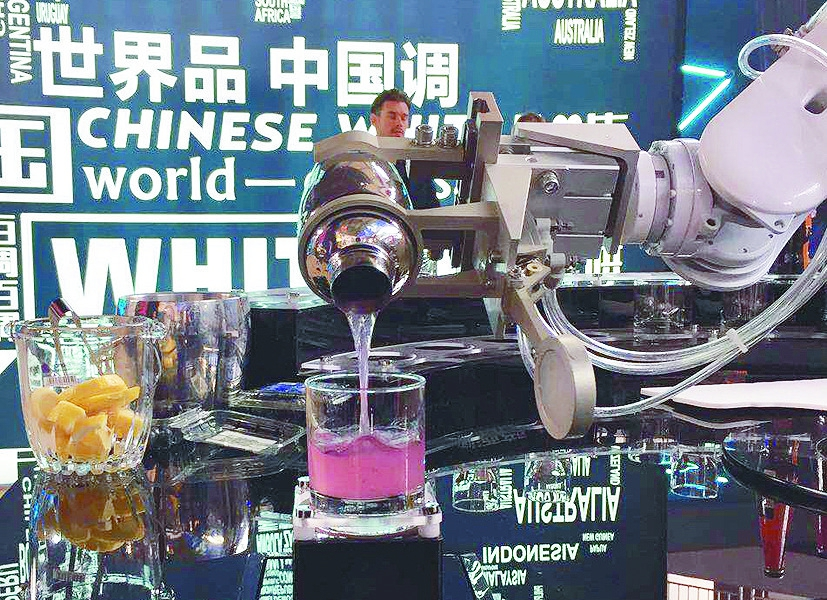
\includegraphics[height=3.5cm]{hgd_arm.jpg}
      \caption{哈工大开发的机器人调酒师}
      \label{fig:hgd_arm}
    \end{subfigure}%
    \caption{机械臂调酒师}
    \end{figure}

\fi

上述这些产品注重控制精度与末端负载,功耗巨大,重量也非常可观,几乎没有移动能力。
尽管工业机器人行业至今已发展多年,体量巨大,技术积累丰厚,但企业的产品研发主要集中在
工业机械臂的硬件性能方面,如提升精度与负载,提升安全性等等。近年来随着电商、物流行业
的迅猛发展,基于机械臂的智能分捡领域开始
蓬勃发展,国内涌现出一批专注物品分捡、分类的创业公司,如深圳蓝胖子机器人~\ref{fig:lanpangzi}、
北京梅卡曼德机器人~\ref{fig:mechmind}等,这些企业专注于算法或者算法硬件集成,致力于
机器人的自动化与智能化。


\begin{figure}
\centering
\begin{subfigure}{.5\textwidth}
  \centering
  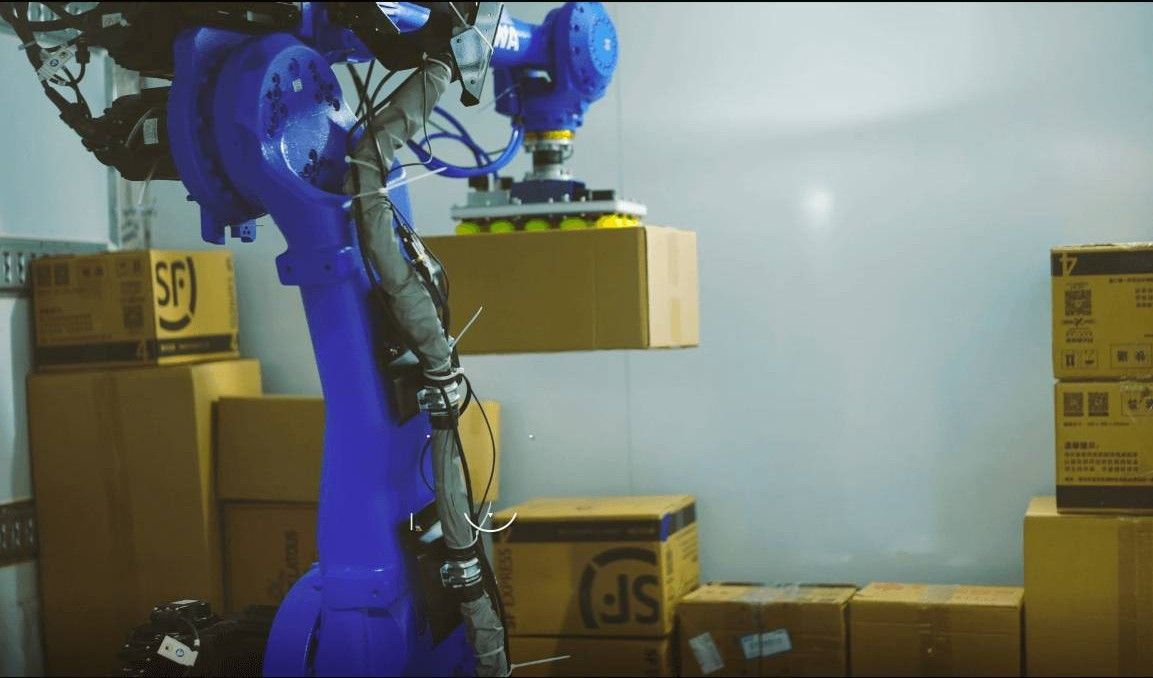
\includegraphics[height=4cm]{lanpangzi_robot.jpeg}
  \caption{蓝胖子机器人研发的机械臂分捡系统}
  \label{fig:lanpangzi}
\end{subfigure}%
\begin{subfigure}{.5\textwidth}
  \centering
  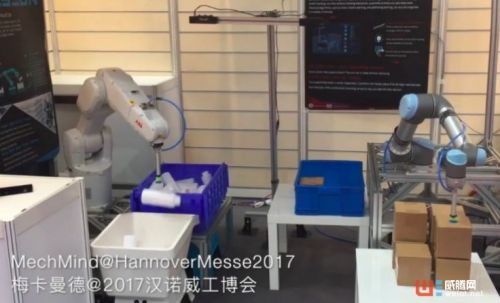
\includegraphics[height=4cm]{mechmind.jpg}
  \caption{梅卡曼德研发的机械臂操作系统在工作}
  \label{fig:mechmind}
\end{subfigure}
\end{figure}

除了专注于操作的工业机械臂,专注移动导航的自动导航车(AGV,Automated Guided Vehicles)
在制造业、运输业也大放异彩。AGV产品最早出现在上世纪50年代,于70年代左右开始应用于
制造业\cite{黄志球2010自动导航车}。按
功能可将AGV分为自动搬运车、自动拖车、自动叉车等几类,或者按照导航方式可分为电磁引导、激光引导、
惯性引导等方式。目前AGV在汽车厂(如通用、丰田、大众等)的制造和装配线上都得到了广泛的使用。
相比于工业机械臂,AGV的机械、电子结构并不复杂,控制算法也相对成熟,制造难度不大。我国的海康威视
就是一个重要的AGV生产商,如图~\ref{fig:haikang}展示了海康威视研发的系列AGV产品。

\begin{figure}
\centering
\begin{subfigure}{.5\textwidth}
  \centering
  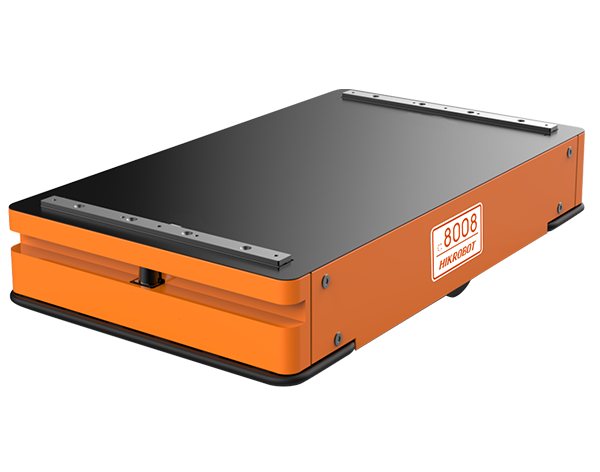
\includegraphics[width=.7\linewidth]{haikang1.png}
  \caption{移载AGV}
\end{subfigure}%
\begin{subfigure}{.5\textwidth}
  \centering
  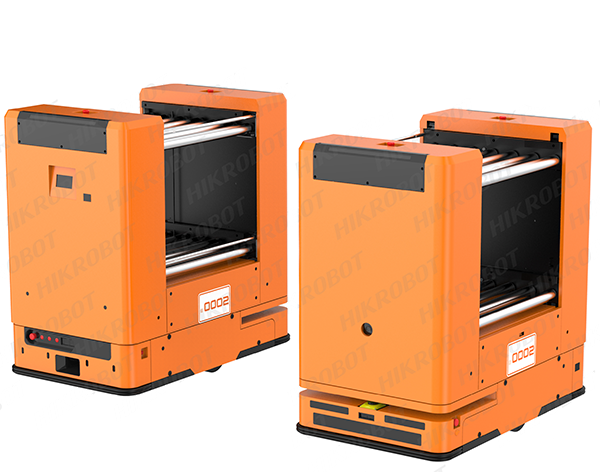
\includegraphics[width=.7\linewidth]{haikang2.png}
  \caption{移载AGV}
\end{subfigure}%
\\
\begin{subfigure}{.5\textwidth}
  \centering
  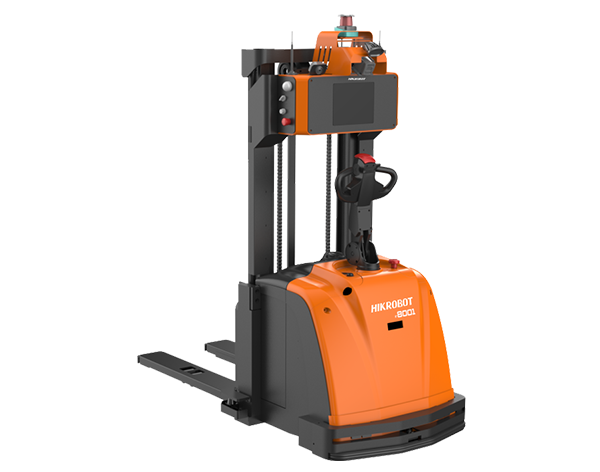
\includegraphics[width=.7\linewidth]{haikang3.png}
  \caption{叉车}
\end{subfigure}%
\begin{subfigure}{.5\textwidth}
  \centering
  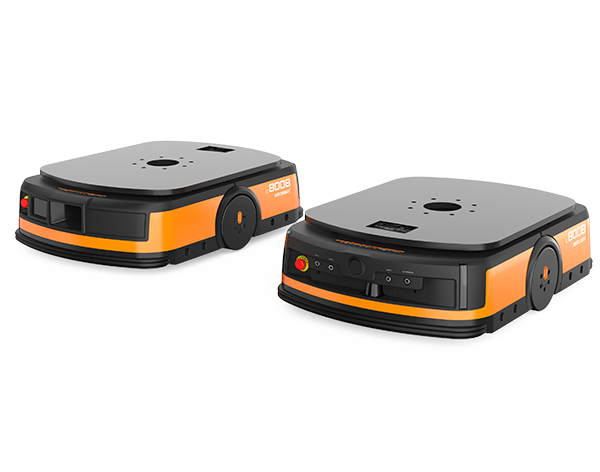
\includegraphics[width=.7\linewidth]{haikang4.png}
  \caption{潜伏系列}
\end{subfigure}%
\caption{海康威视发布的各式AGV产品}
\label{fig:haikang}
\end{figure}

AGV产品除了在制造业广泛应用外,近年来也开始在服务业逐步发展,例如今年来十分火爆的海底捞
机器人餐厅配备了智能AGV送餐员(图~\ref{fig:haidilao}),瑞幸咖啡尝试的无人配送小车
(图~\ref{fig:luckin}),
智行者开发的无人自动清扫车(图~\ref{fig:zhixingzhe}), Yogo Robot开发的写字楼包
裹配送机器人(图~\ref{fig:yogo}),极木科技开发的智能车辆搬动机器人(图~\ref{fig:jimu})
等等。这些产品专注细分领域的需求,有一定的智能处理能力。

\begin{figure}
\centering
\begin{subfigure}{.5\textwidth}
  \centering
  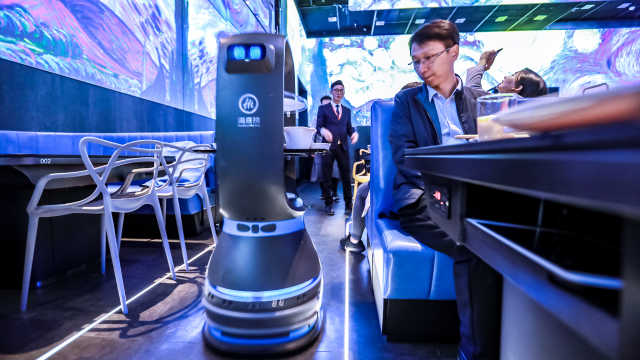
\includegraphics[height=3.5cm]{haidilao.jpg}
  \caption{海底捞送餐机器人}
  \label{fig:haidilao}
\end{subfigure}%
\begin{subfigure}{.5\textwidth}
  \centering
  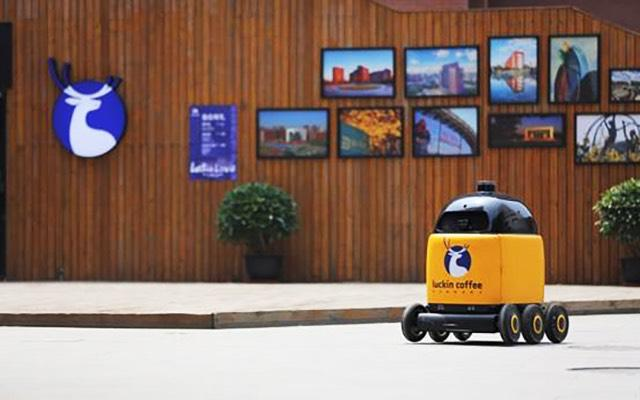
\includegraphics[height=3.5cm]{luckin.jpg}
  \caption{瑞幸咖啡的无人配送车}
  \label{fig:luckin}
\end{subfigure}%
\\
\begin{subfigure}{.5\textwidth}
  \centering
  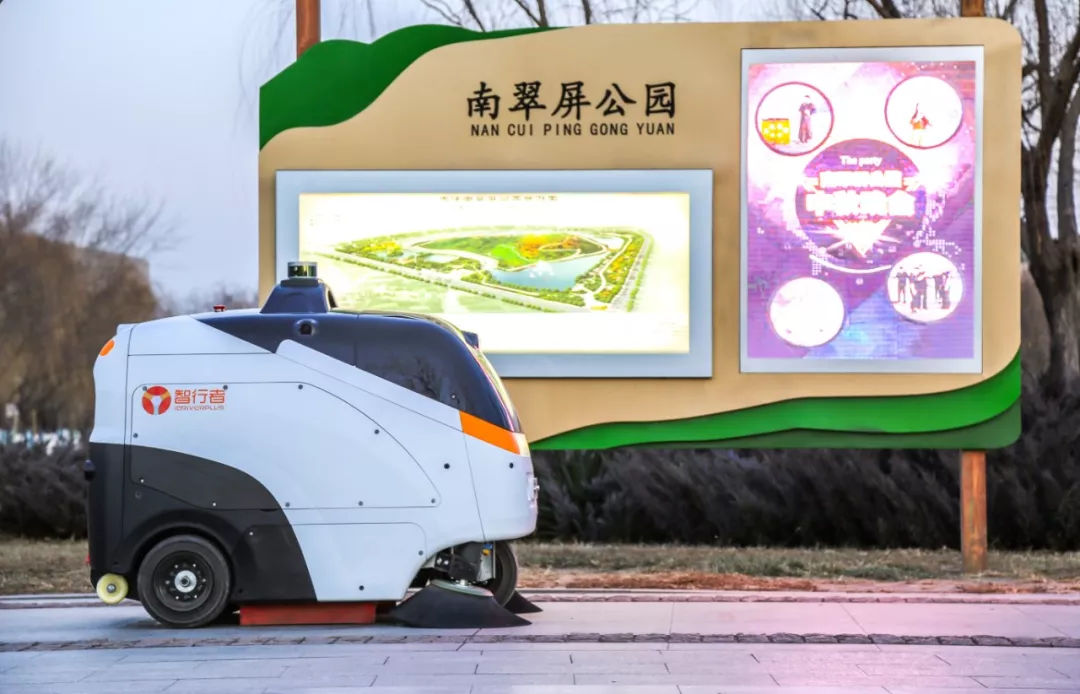
\includegraphics[height=3.5cm]{zhixingzhe.jpg}
  \caption{智行者开发的无人自动清扫车}
  \label{fig:zhixingzhe}
\end{subfigure}%
\begin{subfigure}{.5\textwidth}
  \centering
  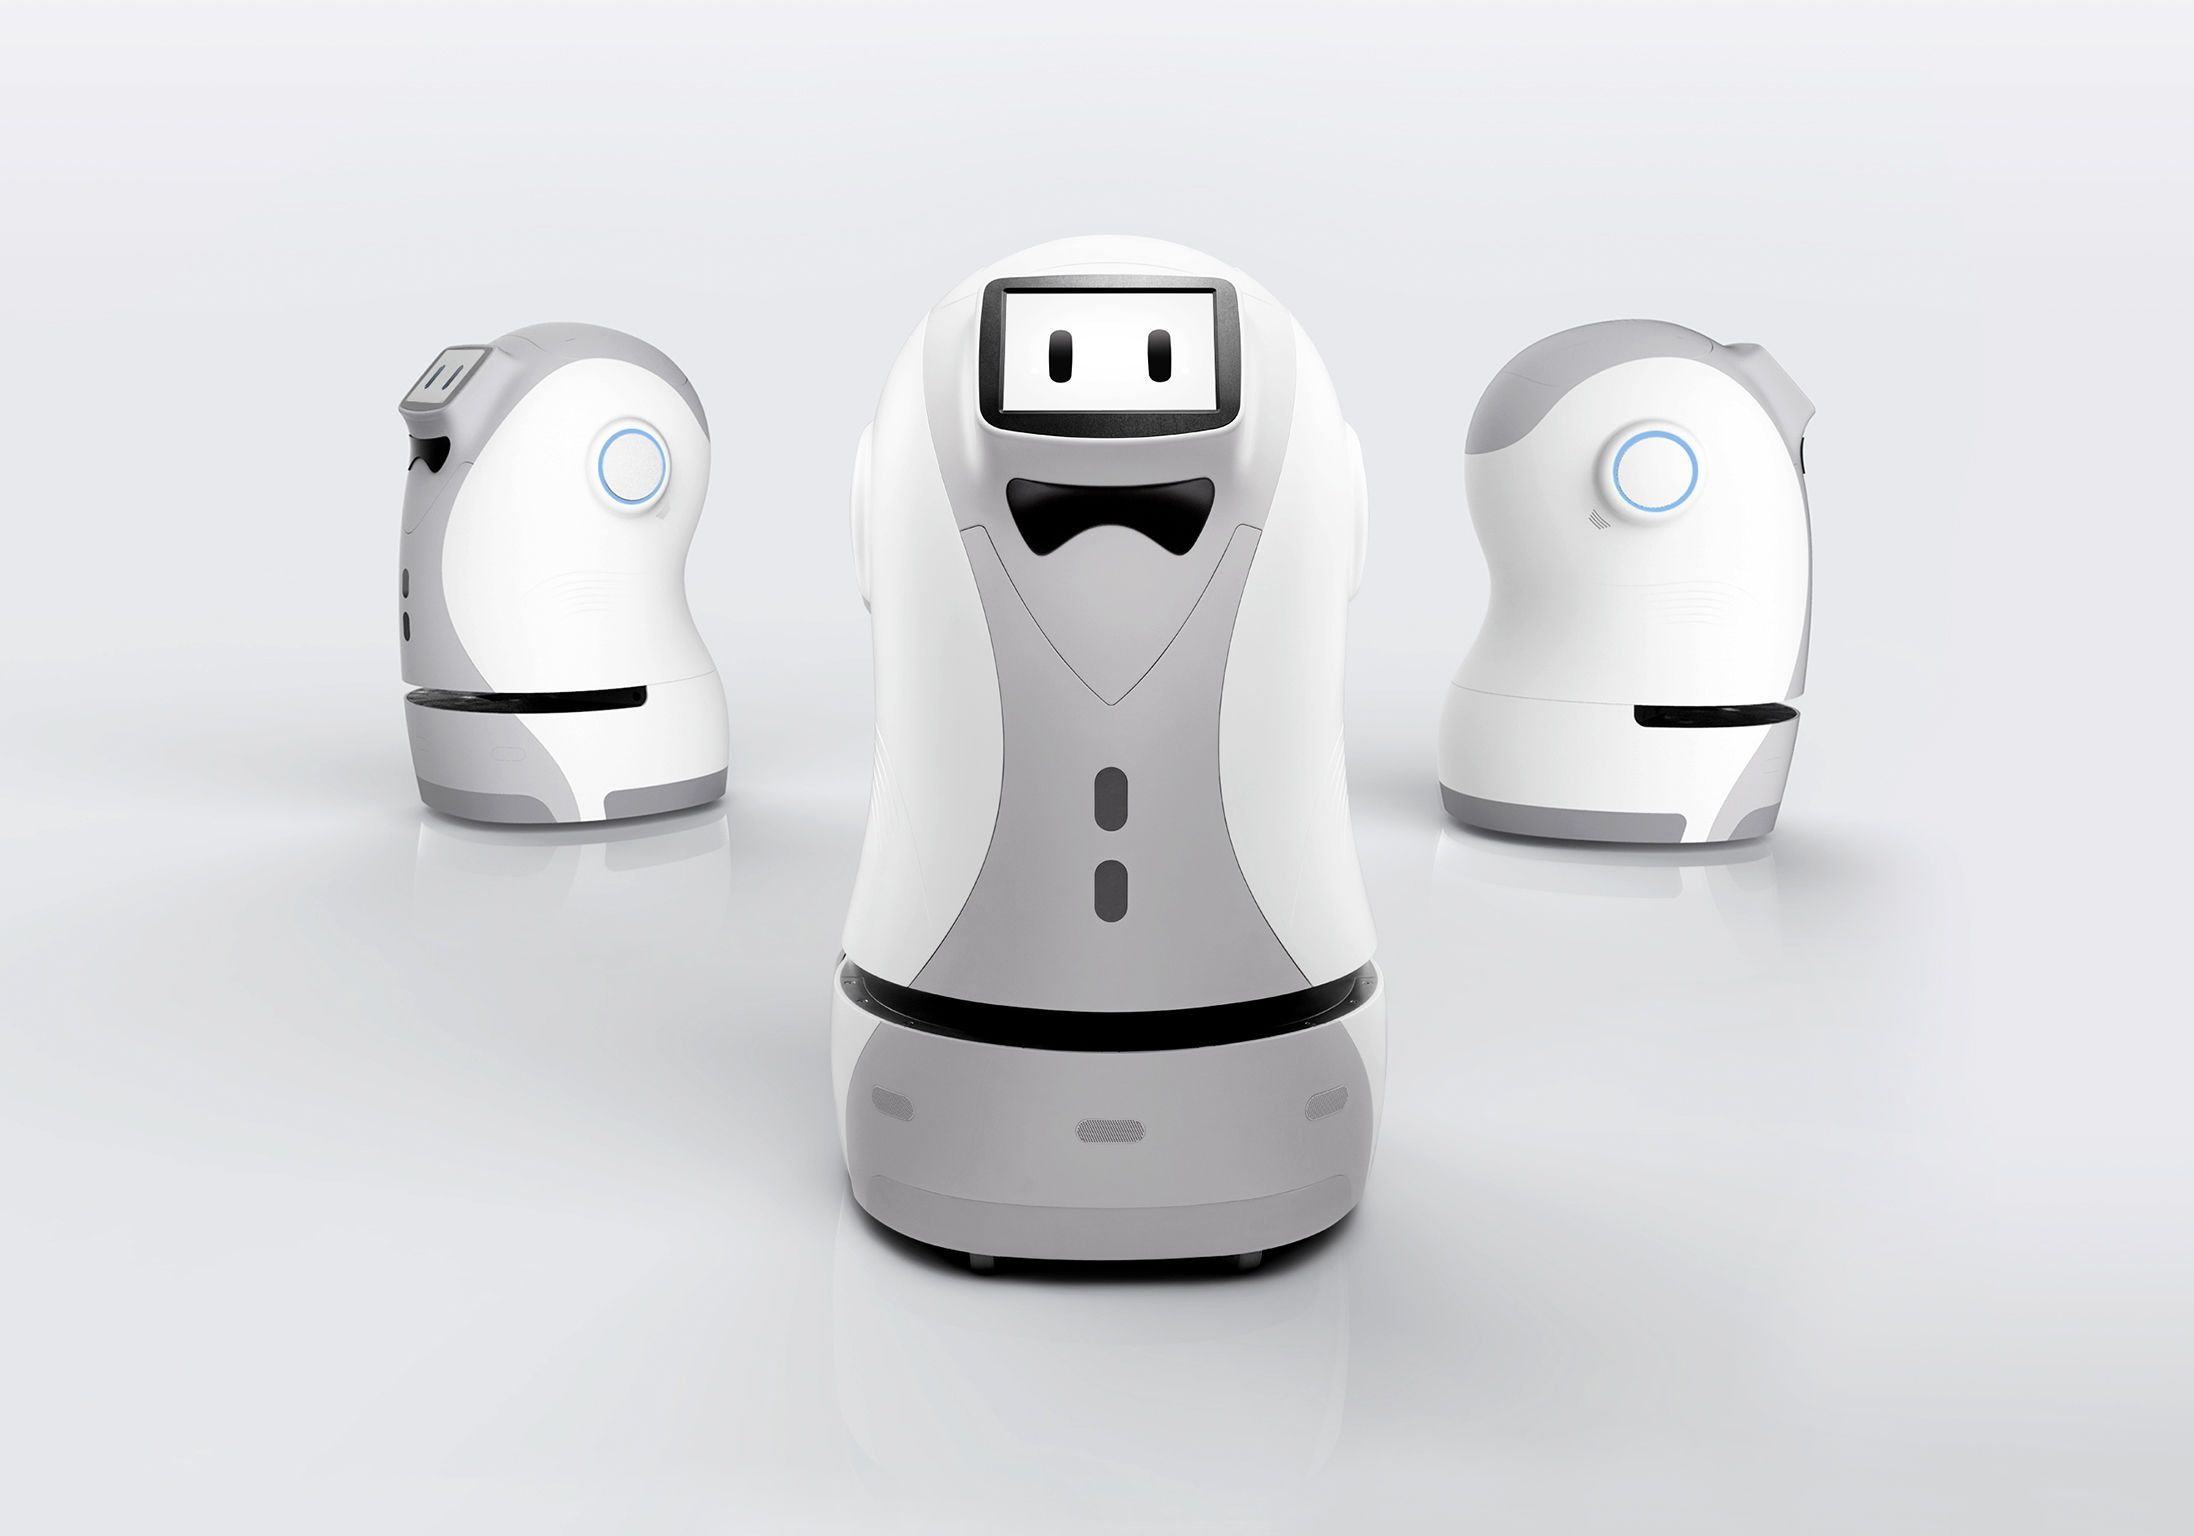
\includegraphics[height=3.5cm]{yogo.jpg}
  \caption{Yogo Robot开发的写字楼包裹配送机器人}
  \label{fig:yogo}
\end{subfigure}%
\\
\begin{subfigure}{.5\textwidth}
  \centering
  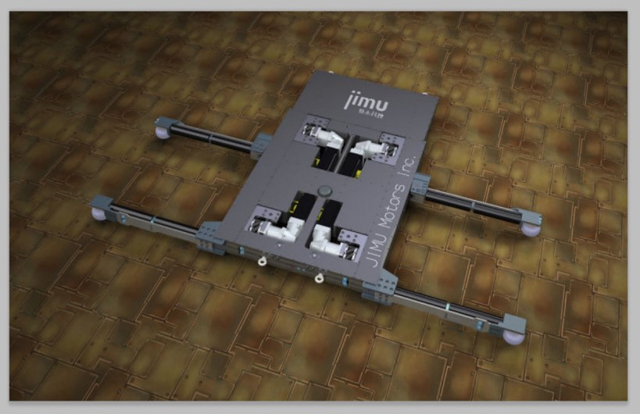
\includegraphics[height=3.5cm]{jimu.jpg}
  \caption{极木科技开发的智能车辆搬动机器人}
  \label{fig:jimu}
\end{subfigure}%
\caption{AGV机器人在服务业的应用}
\end{figure}


移动操作机器人本质上是机械臂产品与AGV的集合,但目前来看其商业应用方向与前两者有极大的区别。
现阶段移动操作机器人领域还没有出现在商业上十分成功的厂商,但是国内外出现了一大批专注这一
领域的创业公司和项目,致力于将移动操作机器人应用到医疗、服务、制造等场景下。例如Diligent Robotics
研发的机器人护士Moxi(如图~\ref{fig:moxi})专注于医院场景下的配送、运输业务;欧
盟发起的旨在推动工业环境中机器人与人写作的”第二双手“(SecondHand)项目的一期项目成
果,AMRAR-6机器人(如图~\ref{fig:armar6})能够在工业环境下与工人协作完成物品的搬动、维修等任务。

\begin{figure}
\centering
\begin{subfigure}{.5\textwidth}
  \centering
  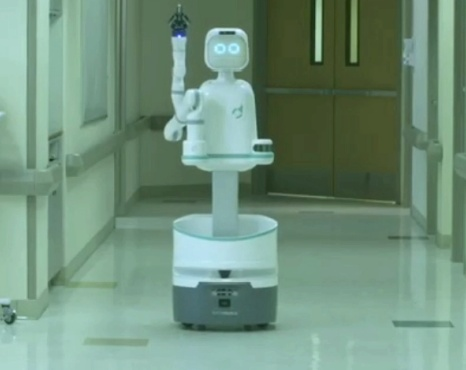
\includegraphics[height=4.2cm]{moxi.jpg}
  \caption{Moxi机器人护士}
  \label{fig:moxi}
\end{subfigure}%
\begin{subfigure}{.5\textwidth}
  \centering
  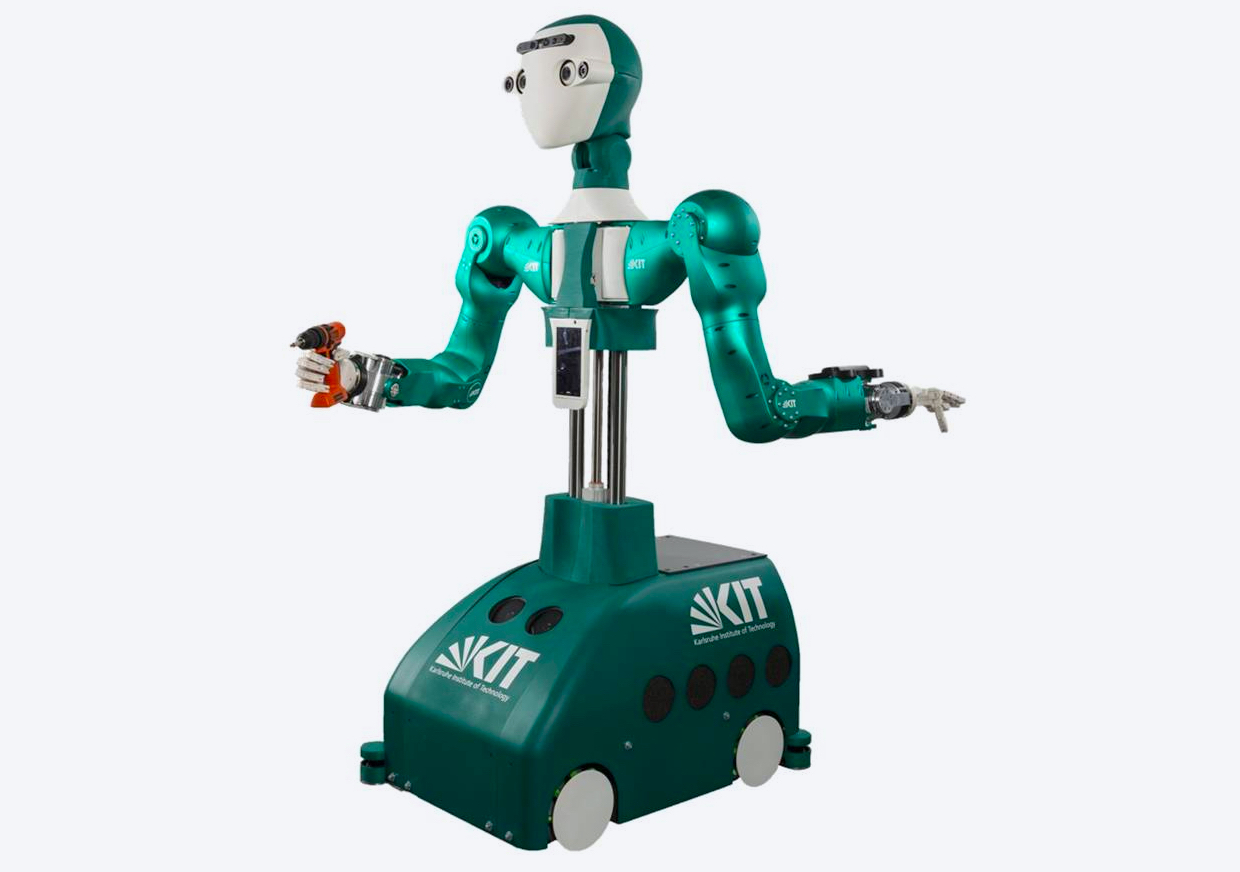
\includegraphics[height=4.2cm]{armar6.jpeg}
  \caption{ARMAR-6仿人机器人}
  \label{fig:armar6}
\end{subfigure}%
\caption{国内外创业公司研发的医疗移动操作机器人}
\end{figure}

除上述两例面向特定任务的移动机器人外,产业界还有一部分产品定位为“仿人”的具有社交属性的服务
机器人,例如日本Toyota公司面对人口老龄化现象推出的家庭照料机器人HSR(Human Support Robot)\ref{fig:hsr},
以及Softbank Robotic发布的Pepper机器人\ref{fig:pepper}。这些机器人大都行动笨拙,但是有双臂、
手、头等和人类身体结构对应的机械结构,并且有一定的交互能力。

\begin{figure}
\centering
\begin{subfigure}{.5\textwidth}
  \centering
  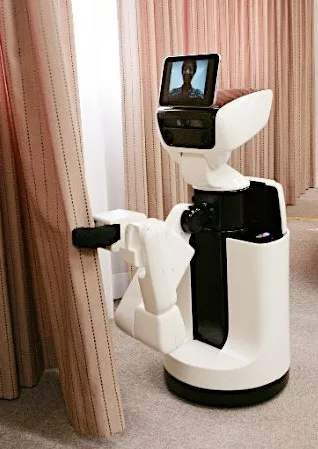
\includegraphics[height=5cm]{hsr.jpeg}
  \caption{Toyota Human Support Robot}
  \label{fig:hsr}
\end{subfigure}%
\begin{subfigure}{.5\textwidth}
  \centering
  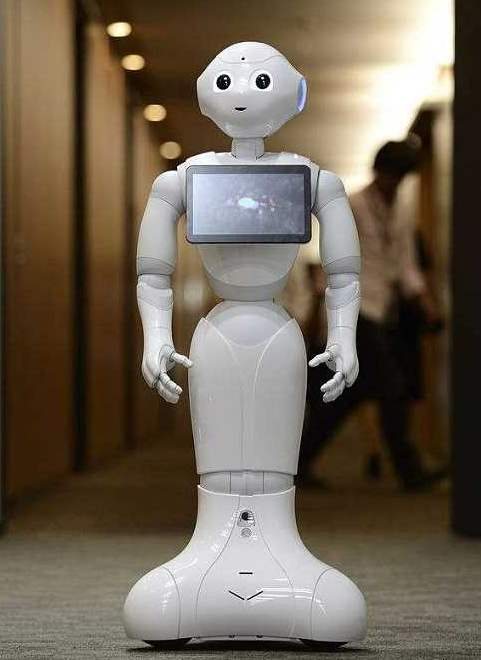
\includegraphics[height=5cm]{pepper.jpeg}
  \caption{Softbank Robotics Pepper}
  \label{fig:pepper}
\end{subfigure}
\label{fig:hsr_pepper}
\caption{仿人机器人产品}
\end{figure}

除了上述商业应用比较明确的公司以及产品外,国际上大名顶顶的波士顿动力公司(Boston Dynamics)也
研究发布了几款轮式移动操作机器人(如图~\ref{fig:bd_wheel}),和以大狗为移动平台挂载轻量
级机械臂的机器人(如图~\ref{fig:bd_dog})。这些机器人在运动控制上均达到了极高的水平,为
移动操作机器人的运动性能评价设定了新的标杆。

\begin{figure}
\centering
\begin{subfigure}{.5\textwidth}
  \centering
  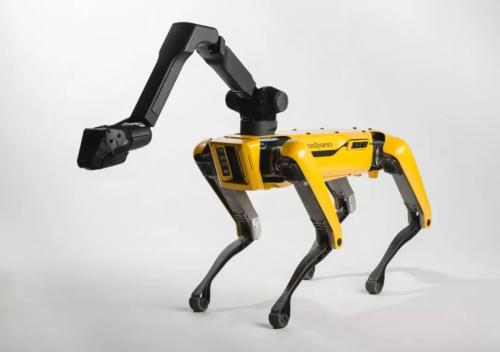
\includegraphics[width=.6\linewidth]{bd_dog.jpg}
  \caption{SPOTMINI + Arm大狗机器人}
  \label{fig:bd_dog}
\end{subfigure}%
\begin{subfigure}{.5\textwidth}
  \centering
  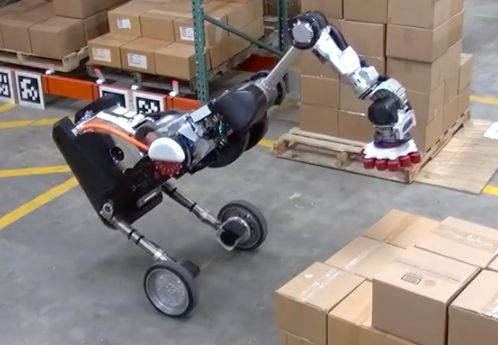
\includegraphics[width=.6\linewidth]{bd_wheel.jpg}
  \caption{仓储搬运机器人Handle}
  \label{fig:bd_wheel}
\end{subfigure}
\caption{波士顿动力发布的移动操作机器人产品}
\end{figure}


\section{移动操作机器人国内外研究现状}
\label{cha:research}

机器人领域中学术界的研究总是走在工业界前面,移动操作机器人方向也不例外。最早的工业
机械臂于1969年由Victor Scheinman发明,称为“斯坦福机械臂”,随后Victor Scheinman在
MIT AI Lab设计了被成为“MIT arm”的机械臂并在一些公司的支持下开发了Puma机器人\cite{huangxihuanReview},
机器人最初诞生自高校的实验室里。在50年后的今天,学术界的研究依然指引着机器人发展的
方向。随着计算机技术的不断发展,深度学习以及各类控制算法的成熟,研究者们开始将目光
聚焦于提升机器人的“智能性”以及它的泛化性上。

学术领域在探索各式感知、控制、交互方法的同时,也自研或者培育了许多移动操作机器人产品。
这些产品机器人不但对领域内前沿的设计思想进行实践、对前沿的传感器进行尝试,方便了广大
研究人员,有些甚至取得了商业上的成功。例如在开源机器人领域著名的PR2机器人
(如图~\ref{fig:pr2})以及TurtleBot(如图~\ref{fig:turtlebot})机器人平台。

\begin{figure}
\centering
\begin{subfigure}{.6\textwidth}
  \centering
  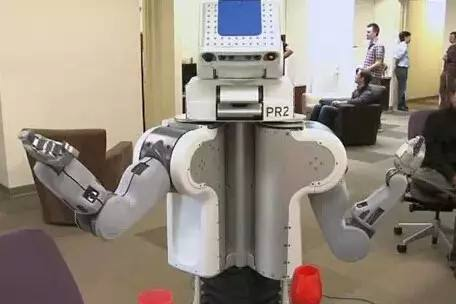
\includegraphics[height=4cm]{pr2.jpeg}
  \caption{PR2服务机器人}
  \label{fig:pr2}
\end{subfigure}%
\begin{subfigure}{.4\textwidth}
  \centering
  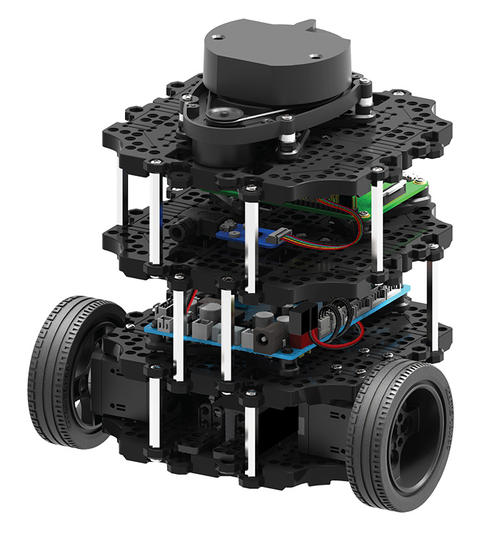
\includegraphics[height=4cm]{turtlebot3.jpg}
  \caption{turtlebot3机器人}
  \label{fig:turtlebot}
\end{subfigure}
\caption{学术机器人平台}
\end{figure}

为了统一机器人算法研究的编程平台,降低方法的复现难度,促进社区的健康发展。广大机器人
研究学者们也参与推动维护了多个开源的机器人编程框架,其中包括应用广泛的ROS
(Robot Operating System)\cite{quigley2009ros},YARP
(Yet another robot platform)\cite{metta2006yarp}等框架。这些开源框架为社区提供了
极大的发展便利,同时某些面向学术研究的移动机器人操作平台也通过捆绑支持这些机器人
编程框架取得了商业上的成功,例如前文提到的PR2和TurtleBot机器人;Universal Robotics
研发的URx系列机械臂(图~\ref{fig:urx}); 以及国内的autolabor四轮
差速车(图~\ref{fig:autolaborpro1} ~\ref{fig:autolabor})等等产品。


\begin{figure}
\centering
\begin{subfigure}{.6\textwidth}
  \centering
  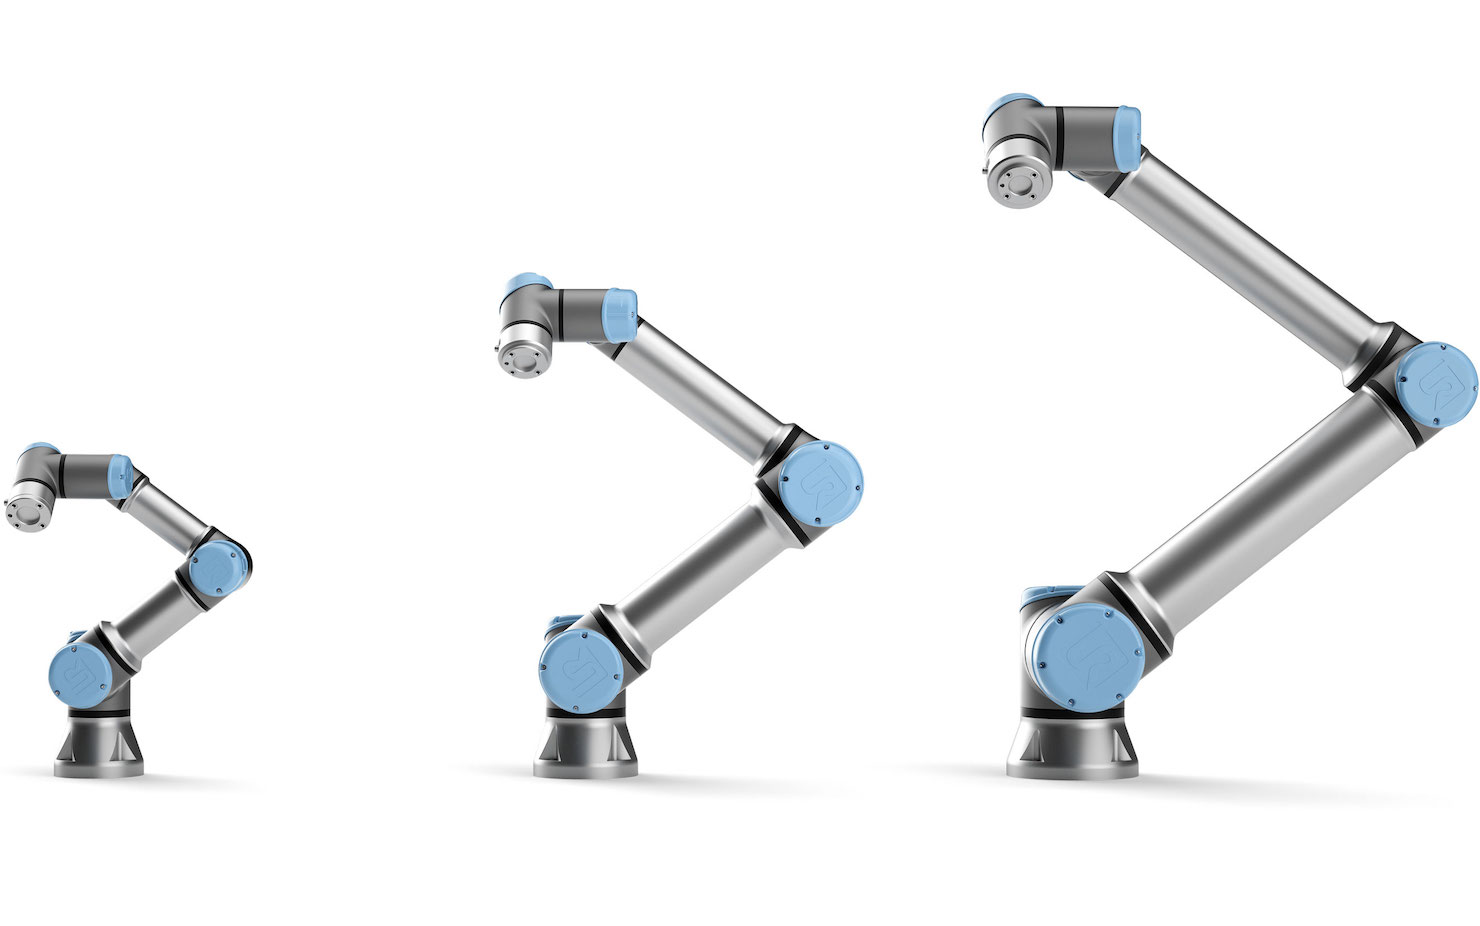
\includegraphics[height=3.5cm]{ur_series.jpg}
  \caption{Universal Robotics研发的系列UR机械臂}
  \label{fig:urx}
\end{subfigure}%
\begin{subfigure}{.4\textwidth}
  \centering
  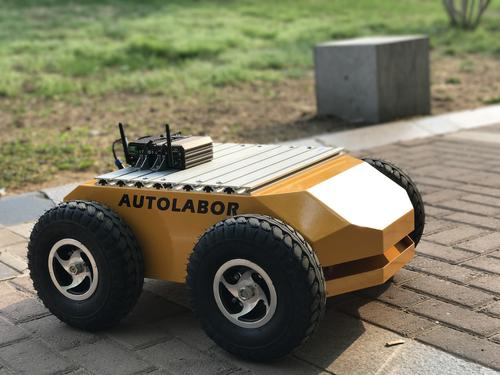
\includegraphics[height=3.5cm]{autolaborpro1.jpg}
  \caption{Autolabor 大负载四轮差速车}
  \label{fig:autolaborpro1}
\end{subfigure}
\begin{subfigure}{.5\textwidth}
  \centering
  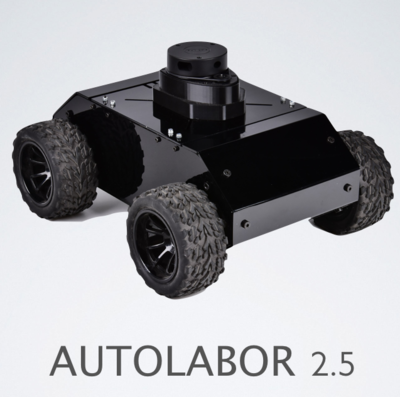
\includegraphics[width=.6\linewidth]{autolabor.jpg}
  \caption{Autolabor小型四轮差速平台}
  \label{fig:autolabor}
\end{subfigure}
\caption{支持ROS平台的机器人产品}
\end{figure}


机器人算法一直是科研领域的研究热点,按照功能可以将机器人相关的算法分为感知和控制两部分。
感知方向包括物品的检测、分类、定位等功能,得益于深度神经网络的快速发展,机器人的感知能力
近年来有了飞速的提高,借助经典的视觉检测方法配合机械臂规划方法实现的快速自动分捡方案
在各大比赛中不断出现。借助深度学习(如图~\ref{fig:img_seg})或者传统视觉方法、点云
处理方法(如图~\ref{fig:pc_seg})实现的拾取平面检测,抓取
点寻找,夹爪位姿寻找算法也不断涌现,并且取得了非常好的效果。

\begin{figure}
\centering
\begin{subfigure}{.5\textwidth}
  \centering
  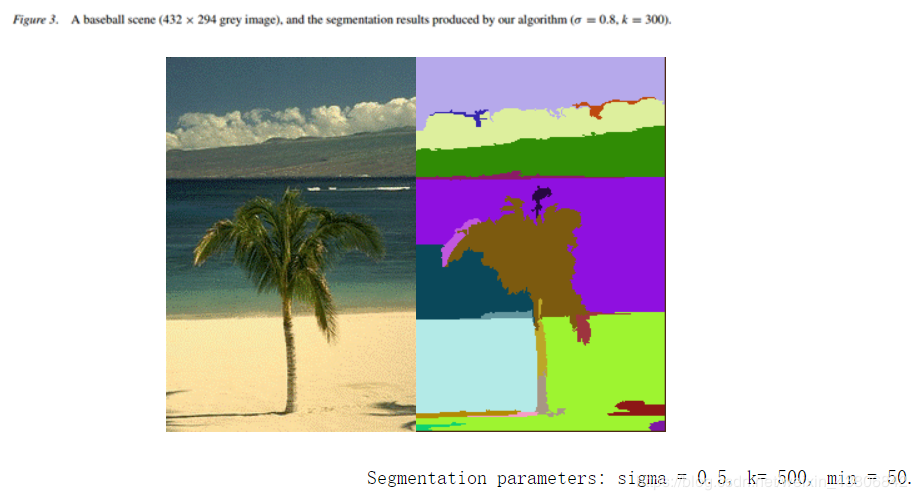
\includegraphics[height=4cm]{img_seg.jpg}
  \caption{基于图片的物品分割识别}
  \label{fig:img_seg}
\end{subfigure}%
\begin{subfigure}{.5\textwidth}
  \centering
  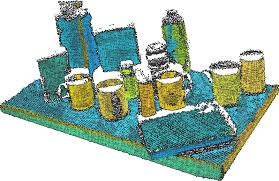
\includegraphics[height=4cm]{pc_seg.jpeg}
  \caption{基于点云的物品分割效果}
  \label{fig:pc_seg}
\end{subfigure}
\caption{学术机器人平台}
\end{figure}


在导航定位方面,SLAM技术( simultaneous localization and mapping,即时定位与地图构建)
日趋成熟,基于视觉、点云或者多传感器融合的算法不断出现,视觉方面,直接法、特征点法
或者半直接的算法大量增加,特别的基于优化的方案有了长足的发展,被认为在未来的SLAM领域能够取代
滤波算法,如基于特征点法的ORB-SLAM\cite{mur2015orb},视觉与IMU融合的VINS\cite{qin2018vins},
半直接法的SVO\cite{forster2014svo},稀疏直接法的DSO\cite{engel2017direct} 等等,
如图~\ref{fig:slams};基于雷达的各类
SLAM算法进展也十分迅速,如基于粒子滤波的Gmapping\cite{grisettiyz2005improving},基于优化
的loam\cite{zhang2014loam},基于优化以及子图的Cartographer\cite{hess2016real}等等。激光
SLAM主要以产出2D地图和位姿为主,其算法结果可视化效果大多很相似,如图~\ref{fig:lidar_slams}

\begin{figure}
\centering
\begin{subfigure}{.6\textwidth}
  \centering
  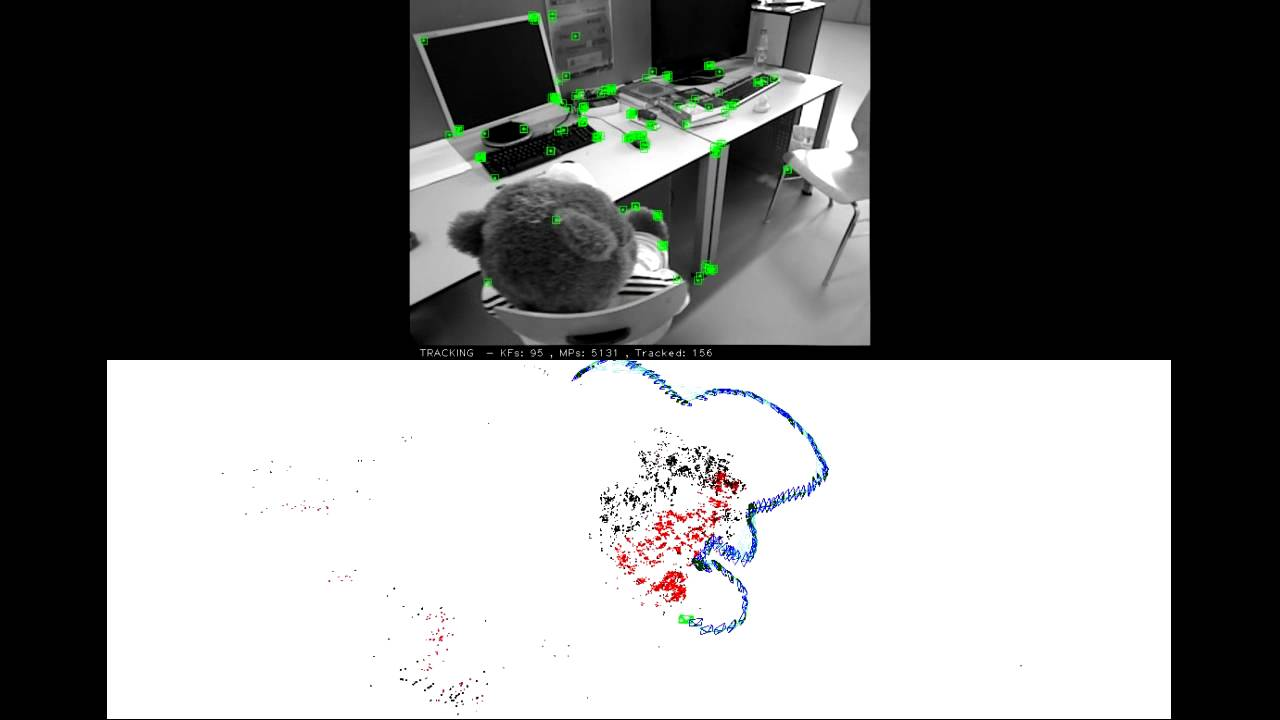
\includegraphics[height=3.5cm]{orb.jpg}
  \caption{ORB-SLAM}
\end{subfigure}%
\begin{subfigure}{.4\textwidth}
  \centering
  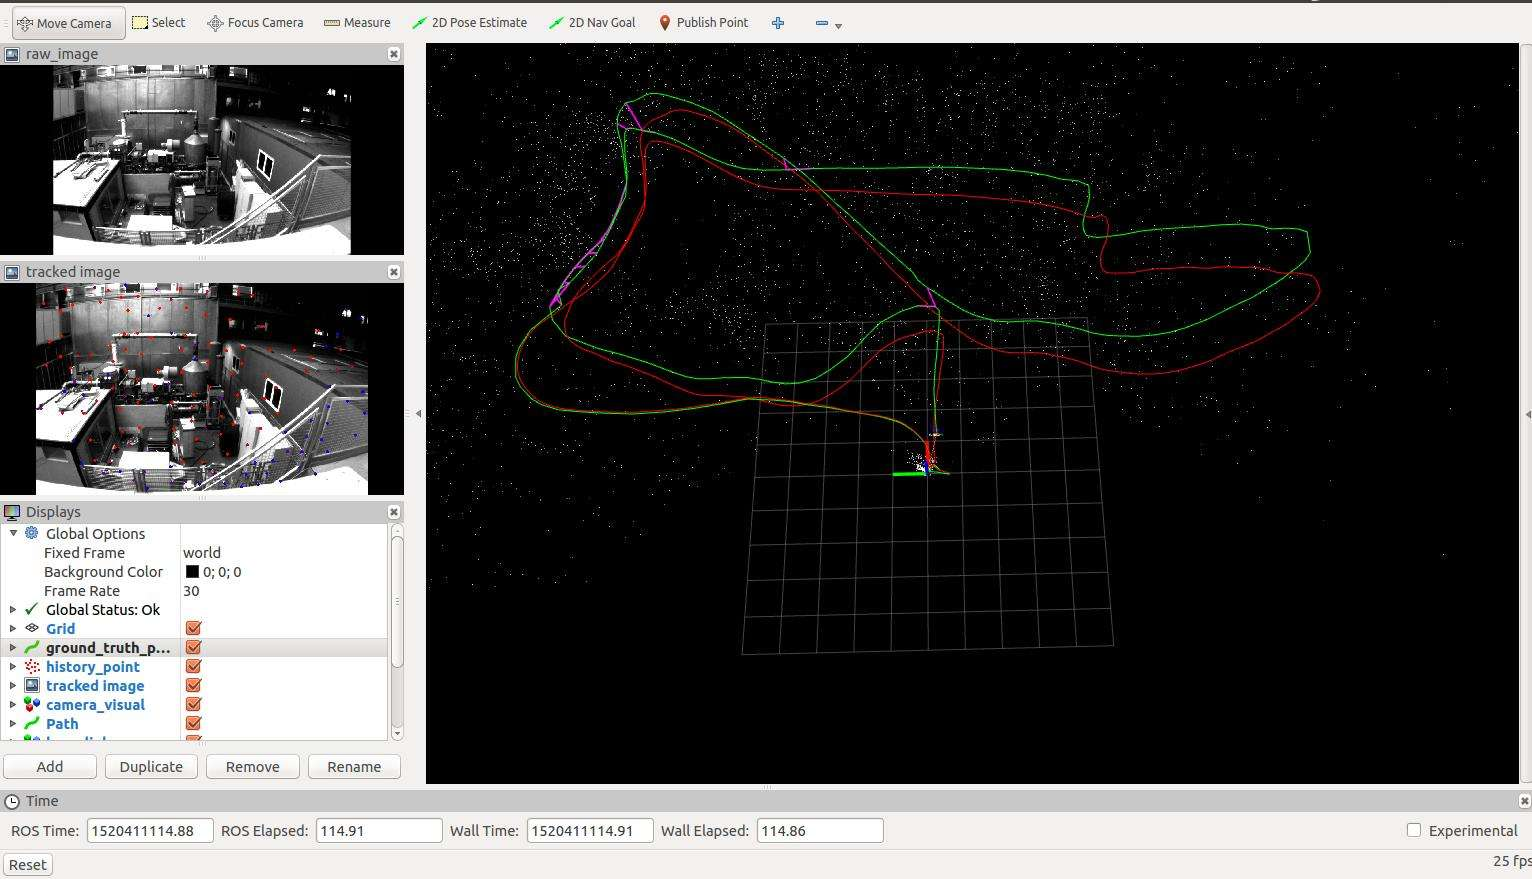
\includegraphics[height=3.5cm]{vins.jpeg}
  \caption{VINS-Mono}
\end{subfigure}
\\
\begin{subfigure}{.59\textwidth}
  \centering
  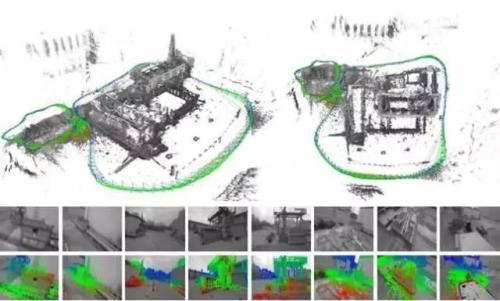
\includegraphics[height=3.2cm]{svo.jpg}
  \caption{SVO}
\end{subfigure}
\begin{subfigure}{.4\textwidth}
  \centering
  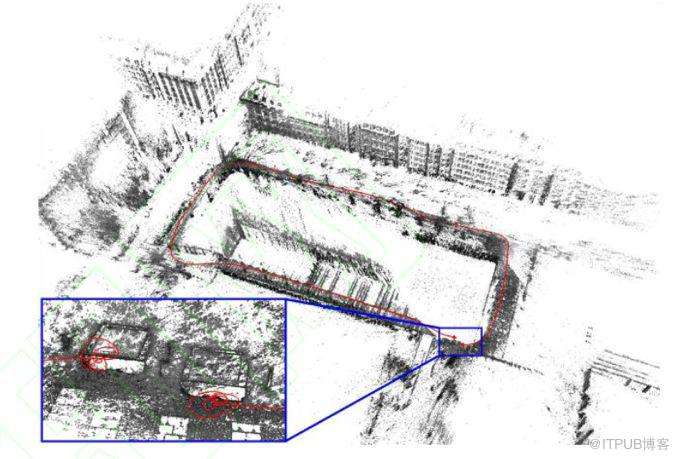
\includegraphics[height=3.2cm]{dso.jpeg}
  \caption{DSO}
\end{subfigure}
\caption{基于视觉的各种SLAM算法效果图}
\label{fig:slams}
\end{figure}


\begin{figure}
\centering
\begin{subfigure}{.5\textwidth}
  \centering
  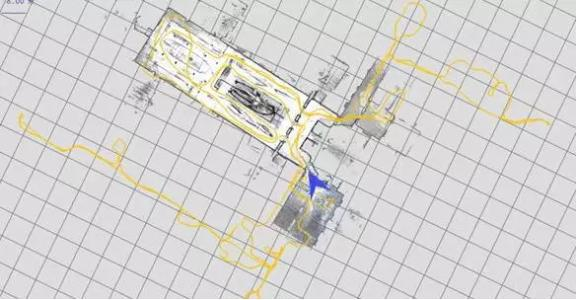
\includegraphics[height=3.7cm]{cartographer.jpg}
  \caption{雷达生成2D地图的可视化效果}
\end{subfigure}%
\begin{subfigure}{.5\textwidth}
  \centering
  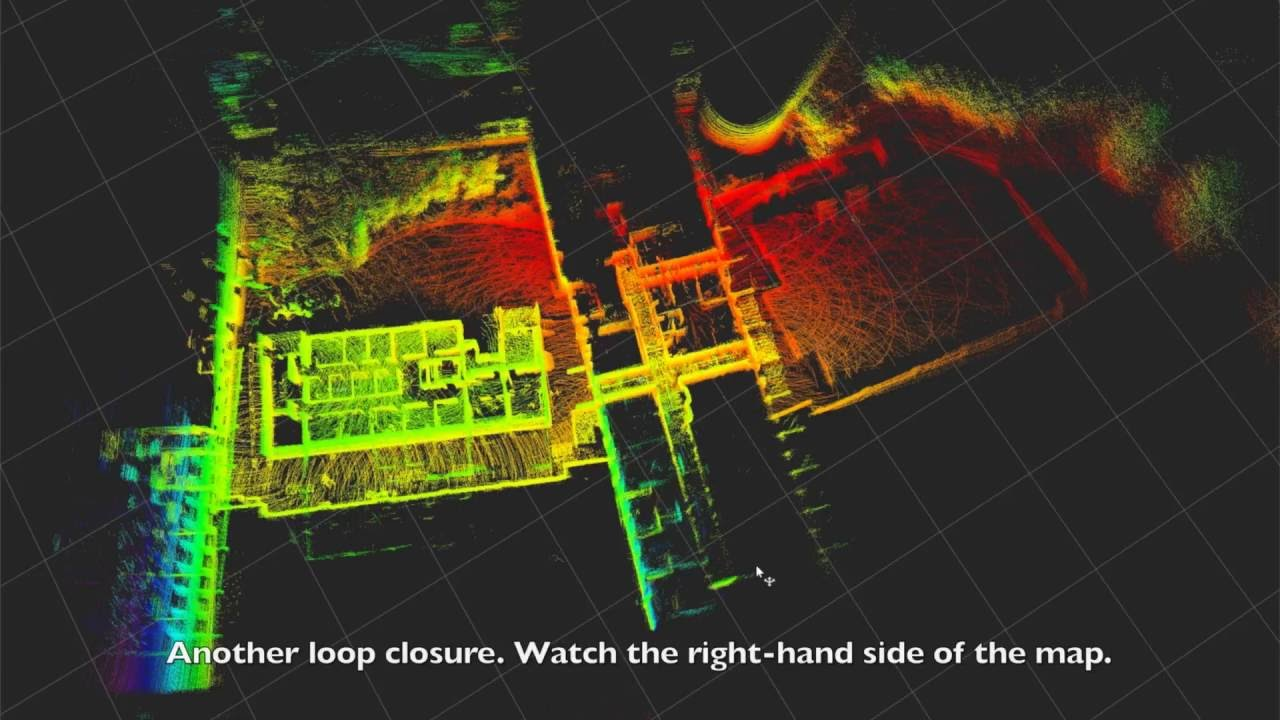
\includegraphics[height=3.7cm]{cartographer3d.jpg}
  \caption{多线激光雷达生成的3D效果图}
\end{subfigure}
\caption{基于雷达的SLAM算法效果图}
\label{fig:lidar_slams}
\end{figure}


格式SLAM算法不断提高机器人主动定位的精度与鲁帮性的同时,导航算法的进步主要体现
在控制框架的创新和完善上,经过数十年的努力,机器人社区在导航方面已经形成了较为稳定的一套
方法,即基于Costmap的分层地图维护方法\cite{lu2014layered}和分别负责路径生成与控制命令
生成的双规划器算法\cite{guimaraes2016ros}。目前
在静态环境中的灵活避障导航问题已经基本被解决\cite{Zhou2017A}。 此外增强学习在机器人控制
上的应用也成为近年来算法方向的研究热点\cite{schaal2002learning}。

机械臂控制算法是机器人算法领域的一大方向,由于现代机械臂自由度高,冗余程度大,状态空间大,
对机械臂的规划算法提出了严峻挑战。学术界不断提出新的机械臂规划算法例如基于梯度优化的机械臂
路径寻找算法 CHOMP\cite{ratliff2009chomp},随机路径优化算法 STOMP\cite{kalakrishnan2011stomp}
等等。同时,一些维护机械臂相关算法 的开源库也迅速兴起,比如维护随机采样规划器的OMPL
(The Open Motion Planning Library)\cite{sucan2010open},
基于搜索算法的SBPL(The Search Based Planning Library)\cite{likhachev2014sbpl},以及
用于碰撞检测的FCL(The Fast Collision Library)\cite{pan2012fcl}。随着这些支撑组件的不断
成熟,一些集运动学解算、路径生成、碰撞检测功能于一体的一站式的机械臂规划框架也开始出现,
如基于ROS的MoveIt!\cite{chitta2012moveit}, V-REP等等,如图~\ref{fig:moveit_vrep}

\begin{figure}
\centering
\begin{subfigure}{.5\textwidth}
  \centering
  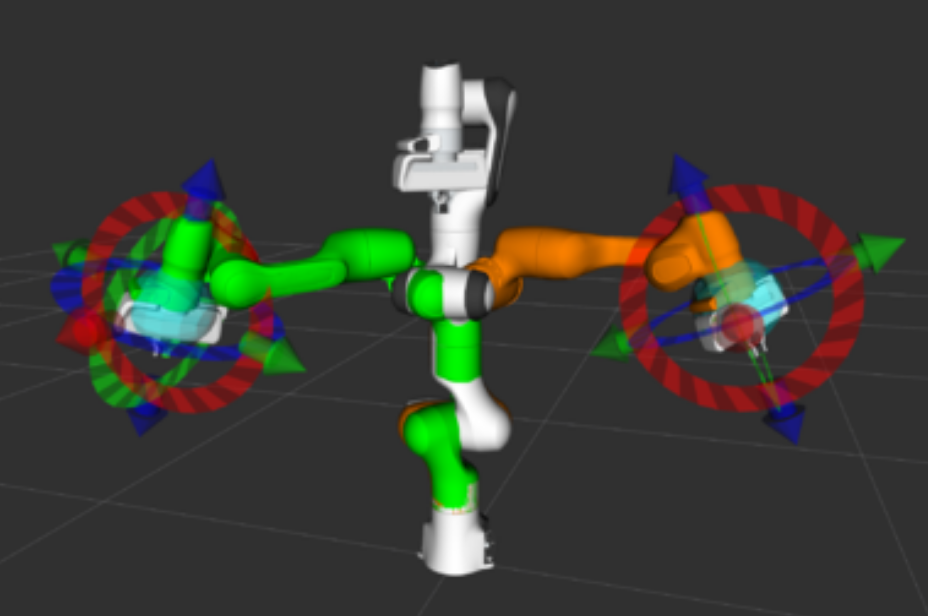
\includegraphics[height=4cm]{moveit.png}
  \caption{MoveIt!工作时的可视化窗口}
\end{subfigure}%
\begin{subfigure}{.5\textwidth}
  \centering
  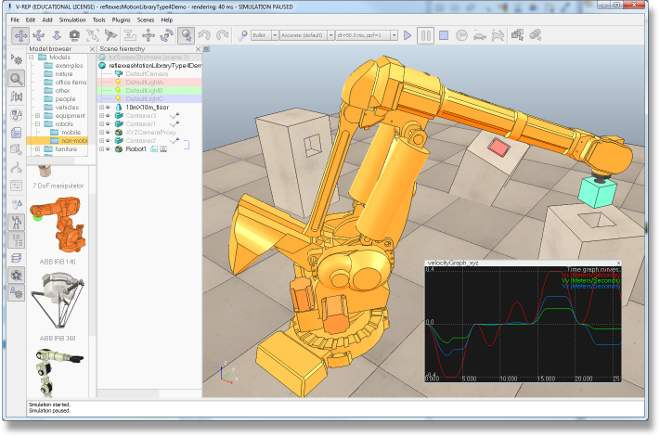
\includegraphics[height=4cm]{vrep.jpeg}
  \caption{V-REP可视化窗口}
\end{subfigure}
\caption{开源的机械臂规划框架}
\label{fig:moveit_vrep}
\end{figure}


为促进研究成果在实际场景中的应用,各大公司会议等组织举办了许多世界级的面向特定场景的
机器人大赛,其中著名的有Amazon Picking Challenge\cite{wurman2016amazon},
RoboCup@Home\cite{wisspeintner2009robocup},IROS Manipulation Competition\cite{moon2017iros}。
这些比赛极大的促进了机器人社区的交流,在比赛期间也涌现出了许多优秀的机器人设计以及
方法。下面以RoboCup@Home为例详细的介绍机器人赛事如何组织及促进学术的发展交流。

RoboCup@Home比赛已经培育起一个完善的社区,每年RoboCup@Home的比赛任务
即由社区相关人员协助商议决定,RoboCup@Home组委会共同维护一份RuleBook\cite{rulebook}
,组委会成员
使用GitHub完成RuleBook的编写任务,该仓库是完全开放且欢迎参赛者提交修改与贡献的。
RoboCup@Home组委会中,设有专门的任务制定部门Technical Committee(TC),这部分成员
大都有深厚的相关从业背景和多年的研究经验,另外有一部分成员来自各个主力参赛队伍的
核心开发人员(比如本文作者作为Tinker机器人的主要程序员参与了2020年的TC工作),以
确保比赛规则同时兼顾学科研究热点和可完成性。

随着机器人行业相关技术的不断发展,RuleBook中的任务也在每年更新,并且向着越来越复杂、
越来越贴近真实生活场景的方向演进。在多年的比赛中,组委会在任务内容、任务形式上也作出
了很多改进与尝试,2019年的RoboCup@Home比赛就及其大胆的将任务数量进行了爆炸式的扩容,
尝试了很多新的复杂的任务,其中有一些被证明并不成功,因此2020年的规则制作过程中又将
不合理的任务去除,将任务数量固定为Stage I 5个,Stage II 4个。 在RoboCup@Home赛场上
出现了大量设计新奇,功能多样的机器人(如图~\ref{fig:other_teams})。

\begin{figure}
    \centering
    \begin{minipage}{.45\linewidth}
            \begin{subfigure}[t]{.9\linewidth}
                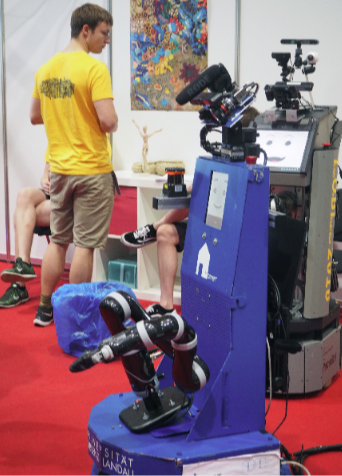
\includegraphics[width=\textwidth]{homer.png}
                \caption{homer@ UniKoblenz}
            \end{subfigure}
    \end{minipage}
    \begin{minipage}{.45\linewidth}
        \begin{subfigure}[t]{.8\linewidth}
            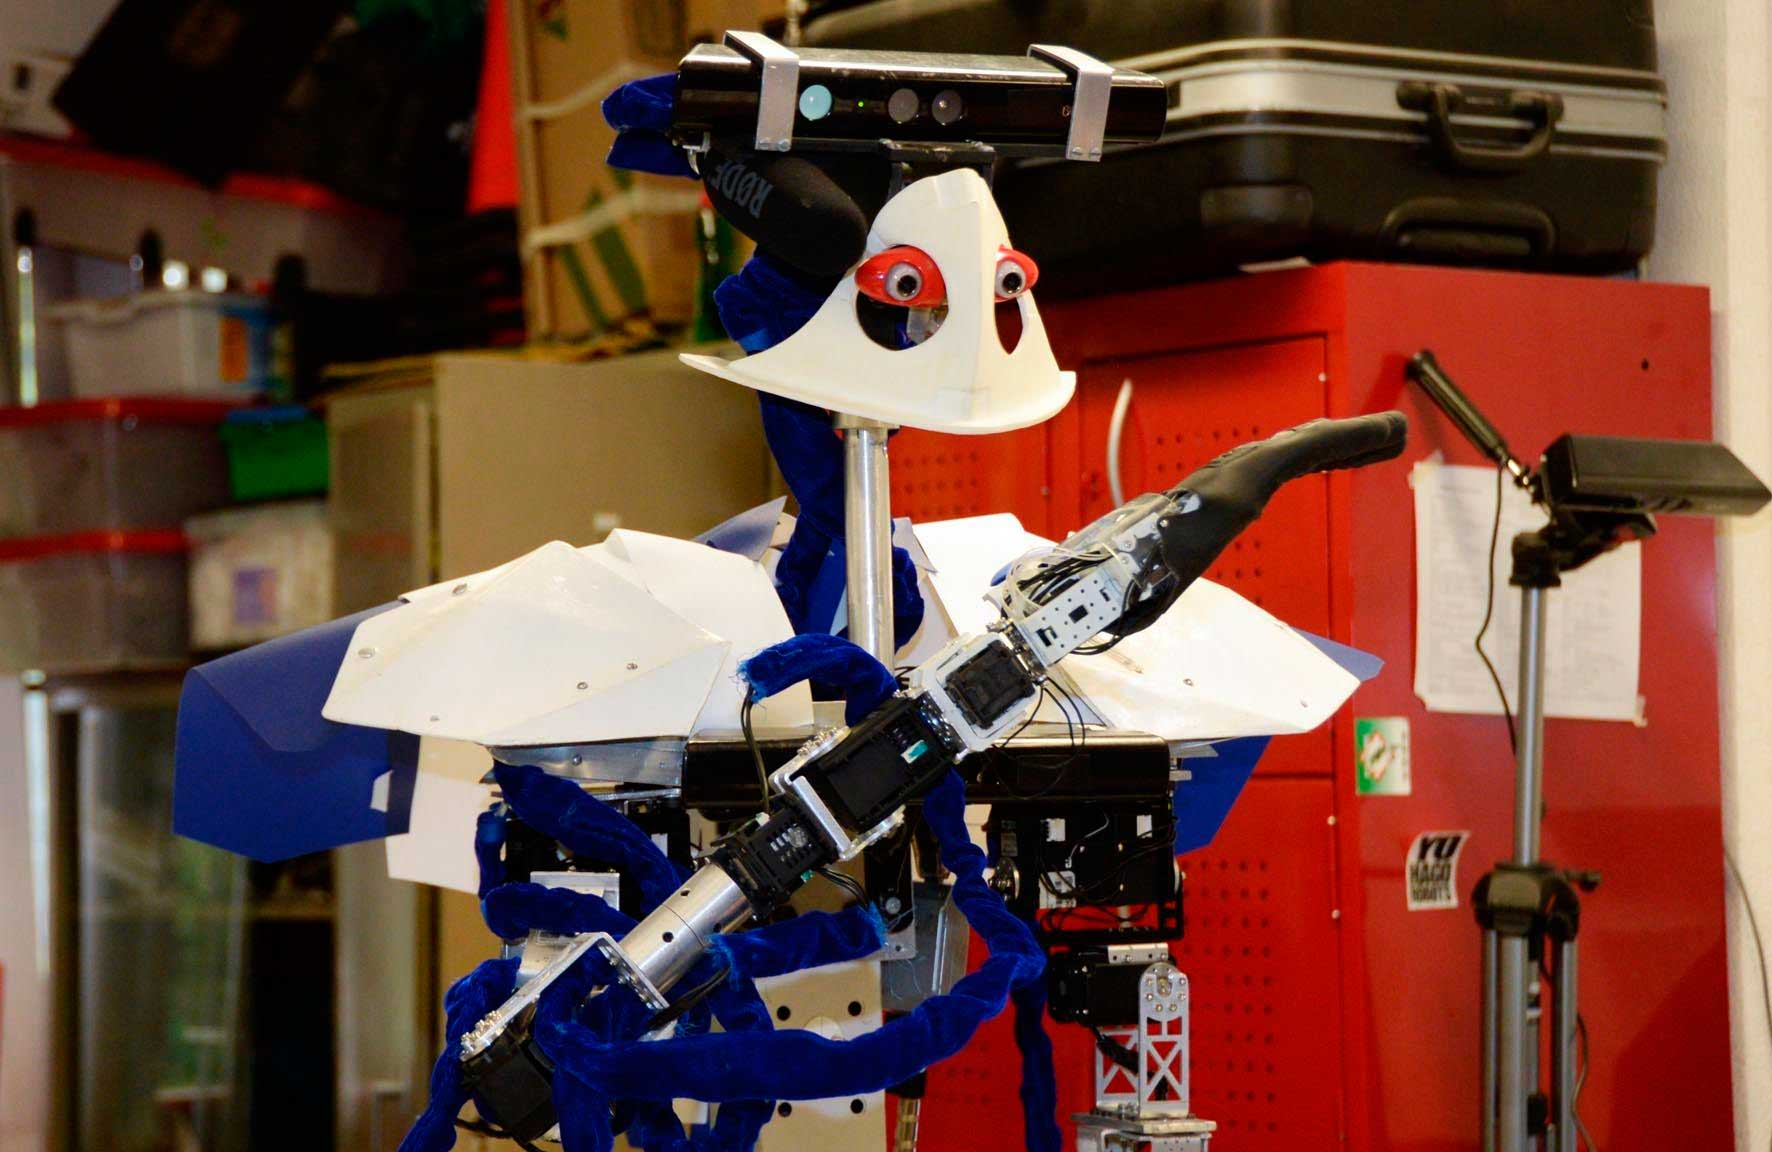
\includegraphics[width=\textwidth]{pumas.jpg}
            \caption{Pumas}
        \end{subfigure} \\
        \begin{subfigure}[b]{.8\linewidth}
            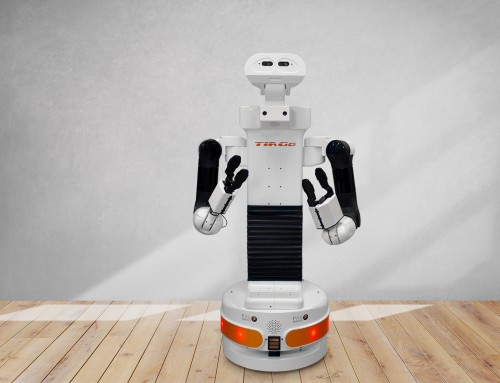
\includegraphics[width=\textwidth]{catie.jpg}
            \caption{CATIE Robotics}
        \end{subfigure} 
    \end{minipage}
    \caption{RoboCup@Home中出现的机器人}
    \label{fig:other_teams}
\end{figure}

\section{本文内容简介}

本章系统的介绍了移动操作机器人的基本定义和国内外研究、应用现状。后续章节将对本文的
主要工作——Tinker移动操作机器人进行介绍,详细的给出Tinker机器人的系统搭建,定位
导航算法的实现与调试,机械臂控制及相应的视觉算法实现以及各部分的版本迭代经过。






% !TeX root = ../main.tex

\chapter{移动操作机器人的系统搭建}
\label{cha:system}


\section{机械结构设计}

按结构划分,可以将Tinker的机械结构粗略的划分为头部,机械臂,骨架,身体主控
以及底盘。机器人的整体外观如图~\ref{fig:tinker_front_side}所示。

\begin{figure}[ht] % use float package if you want it here
  \centering
  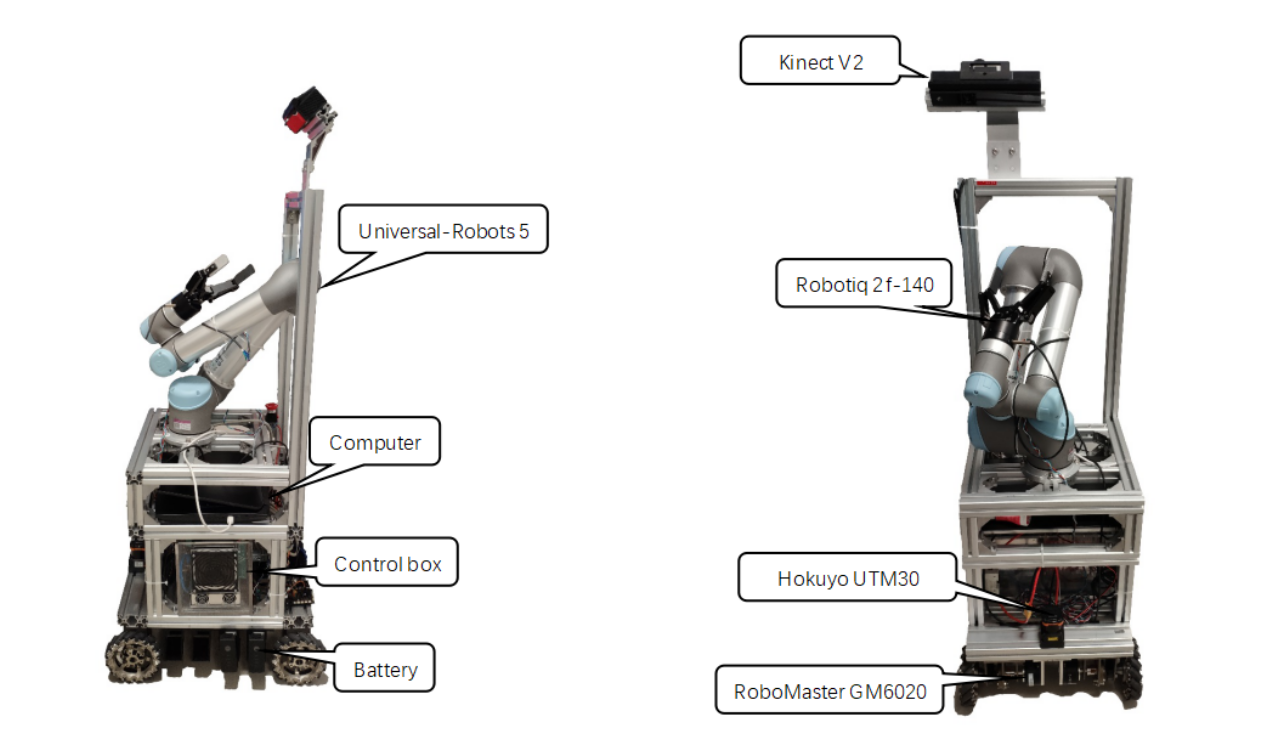
\includegraphics[width=1.\linewidth]{tinker_front_side.png}
  \caption{Tinker前视图与侧视图}
  \label{fig:tinker_front_side}
\end{figure}

\subsection{Tinker骨架搭建}
为方便交通运输与结构迭代,Tinker基本骨架使用40cm*40cm铝形材搭建。骨架
的主要作用为搭建起整个机器人的框架,将各个传感器假设到理想的位置上,并且
为机器人的主控、供电、走线留出足够的空间。经过多轮版本迭代后,目前Tinker
底盘尺寸固定在35cm×45cm,净高140cm,总质量70kg。

为了方便Tinker机器人机械结构长期的维护,降低人员交接成本,我们将Tinker
使用的型材尺寸做了规范化处理,并且对骨架进行了手动建模,以方便机器人的拆
装与改进,如图~\ref{fig:base_link}所示。

\begin{figure}[ht] % use float package if you want it here
  \centering
  \includegraphics[width=.4\linewidth]{base_link.png}
  \caption{Tinker骨架的STL建模结果}
  \label{fig:base_link}
\end{figure}

\subsection{头部设计及版本迭代}

新版的Tinker头部主要用来放置顶部摄像头,在背景环境特别复杂的情况下还会在头部
旁边加装专业的采音麦克风用于语音识别和声源定位。在一般情况下使用头部安装的kinect v2
摄像头自带的麦克风阵列即可满足需求。在Tinker中期我们曾经使用过2自由度云台支持
头部摄像头,使头部摄像头具有上下和左右转动的能力,以扩大摄像头的视野,如图~\ref{fig:neck}
所示。该转台是机器人团队根据现有的通用二自由度转台自行改装的,主要改动有:更换了
原有的舵机,改为精度更高且有位置反馈的dynamixel MX28-AR舵机,
并且相应的改装了转台本身的尺寸和各种装配零件。客观上这一设计确实提高了机器人头部
传感器的视野,但是经过漫长的实践,这一结构被证明是一个彻头彻尾的失败设计。原因有
二:dynamixel本身需要合理的供电和信号线,摄像头本身也有相应的传输线,这些线在频繁
转动的时候很容易被拉断造成整个控制系统崩溃;摄像头本身作为抓取和部分避障的主力
传感器,其位置精度是非常重要的,但是由于舵机空程以及装配过程中产生的空程等等问题,
转台的位置精度一直无法达到要求,大大减弱了摄像头的数据效果。因此在新版的Tinker
中,转台这一设计被机器人团队彻底抛弃了。

\begin{figure}[ht] % use float package if you want it here
  \centering
  \includegraphics[width=.4\linewidth]{neck.png}
  \caption{早期Tinker头部的2自由度转台}
  \label{fig:neck}
\end{figure}

\subsection{Tinker机械臂方案选择}

Tinker使用的机械臂为Universal Robotics公司生产的6自由度机械臂UR5。在决定使用
该机械臂之前我们对市面上在售的各种成品机械臂进行了广泛的调研,包括RoboCup@Home
赛场上使用过的Kinova~\ref{fig:kinova}
机械臂配合三指夹爪,Retinker Robotics公司开发的Sawyer(图~\ref{fig:sawyer})
机械臂,以及Universal Robotics公司出产的各个型号的机械臂(图~\ref{fig:ur_series})。
最终综合考虑了价格、售后、供电、开发者社区等
各个因素后,我们最终确定使用了UR5这个型号的机械臂,并且对机械臂的控制与供电进行了
适当的改装,以符合比赛的需要。

\begin{figure}
\centering
\begin{subfigure}{.5\textwidth}
  \centering
  \includegraphics[width=.9\linewidth]{kinova.png}
  \caption{Kinova}
  \label{fig:kinova}
\end{subfigure}%
\begin{subfigure}{.5\textwidth}
  \centering
  \includegraphics[width=.5\linewidth]{sawyer.jpg}
  \caption{Sawyer}
  \label{fig:sawyer}
\end{subfigure}
\begin{subfigure}{.8\textwidth}
  \centering
  \includegraphics[width=.7\linewidth]{ur_series.jpg}
  \caption{UR系列机械臂}
  \label{fig:ur_series}
\end{subfigure}
\caption{本工作前期调研时关注过得机械臂型号}
\label{fig:arms}
\end{figure}

早期夹爪使用Robotiq
公司生产的Robotiq 2f-85二指夹爪(最大张角85mm),后经过不断的测试与赛场上的较量,
我们发现2f-85的张角对于家庭机器人来说过窄,于是换用了robotiq 2f-140款式的二指夹爪,
该夹爪张角为140mm,能够更好的满足抓取物品、拾取袋子的需求。因此本工作最终使用
UR5 + Robotiq 2f-140作为最终比赛方案,如图~\ref{fig:ur5_2f140}所示。

\begin{figure}[ht] % use float package if you want it here
  \centering
  \includegraphics[width=.4\linewidth]{ur5_2f140.jpeg}
  \caption{Tinker最终使用的机械臂及夹爪方案}
  \label{fig:ur5_2f140}
\end{figure}

\subsection{主控与供电}

Tinker的核心控制由一台搭载了i9-9900K cpu及RTX2080显卡的笔记本电脑完成。在前
几代Tinker设计中,一般主控由工控机或者经过电源改装的台式机担任,但是随着笔记本
性能的不断增强,我们最终选择使用成品机器完成这一任务。成品笔记本性能好,散热完善
且主板设计精良,稳定性好,并且笔记本有自己独立的供电系统,可在机器人断电时单独运行
大大的提升了系统的稳定性和易用性。

整个机器人的供电系统都放在机器人腹部,包括机械臂、底盘、各种传感器、笔记本电脑所需
的所有供电电路以及电池组。2019年Tinker使用单一磷酸铁锂电池供电,标准输出电压29.4V
到24V,容量50AH,放在底盘上部。经过19年比赛的反思之后,作者认为,使用单一锂电池
供电太过危险,且参赛过程中运输太过麻烦,成本过高,于是我们将供电方案改成了多块标准
29V 1500mAH电池并接供电的形式,并3D打印了特制的电池架将电池倒挂在底盘下,这样一方面
大大缩小了Tinker底盘的面积提高了底盘避障导航的灵活性,另一方面降低了整个机器人的中心,
使得机械臂运动时的型变更小,提高了机器人的性能。在供电电路布线方面,Tinker也有了
显著的改进,前一版本中Tinker直接借用了UR5自带的配电箱摆放机械臂及其他部件需要的
供电线路、DCDC、分流排等等元件。但是配电箱本身尺寸过大,不透明,且强度过大,给机器人
装配、调试带来了很大的困难,也对导航的表现造成了影响。之后我们在充分考虑了散热、消防
等等制约之后,使用亚克利版重新制作了一版配电箱,且对机器人的供电线路进行了梳理,大大
缩小了机器人的底盘尺寸,也使得整个供电设计更加简洁易于调试。前后两个版本的供电外观
如图~\ref{fig:elec}所示。

\begin{figure}
\centering
\begin{subfigure}{.5\textwidth}
  \centering
  \includegraphics[height=6cm]{tinker_elec.jpg}
  \caption{改版前的电池及供电线路放置}
  \label{fig:old_elec}
\end{subfigure}%
\begin{subfigure}{.5\textwidth}
  \centering
  \includegraphics[height=6cm]{tinker_elec_new.jpg}
  \caption{改版后的电池及供电线路放置}
  \label{fig:new_elec}
\end{subfigure}
\caption{Tinker前后两个版本的供电布局}
\label{fig:elec}
\end{figure}

\subsection{底盘设计}

Tinker的底盘设计受前几版机器人的影响最多,早期的Tinker使用自制的3自由
度机械臂,其精度有限且自由度受限太严重,需要具有左右额外自由度的底盘
来弥补这一不足,因此Tinker的底盘被设计为使用4个麦克纳母轮的万向底盘
\cite{tlale2008kinematics},底盘设计如图~\ref{fig:chassis_sw}所示,
由于我们使用的麦轮为标准成品,因此在设计图中将麦轮的细节全部简化了。

\begin{figure}[ht] % use float package if you want it here
  \centering
  \includegraphics[width=.7\linewidth]{chassis_sw.png}
  \caption{Tinker底盘悬架的SolidWorks设计图}
  \label{fig:chassis_sw}
\end{figure}

新版Tinker改为成品机械臂后抓取的自由度和覆盖范围都有了质的飞跃,不再要求
底盘具有万向移动的性能了。但是经过多年的改进,机器人团队中对万向底盘的制作
技术已经成熟,于是我们继续沿用了这一设计,仅在电机选型上做了一些与时俱进
的改良,选用了扭矩较大且噪音较小的大疆 GM6020直流无刷电机做底盘的动力电机,
如图~\ref{fig:chassis}所示。

\begin{figure}[ht] % use float package if you want it here
  \centering
  \includegraphics[width=.7\linewidth]{chassis.png}
  \caption{Tinker底盘的电机传动结构}
  \label{fig:chassis}
\end{figure}


\section{电路设计及通信设计}

Tinker机器人作为一个有复杂功能和结构的完整机器人系统,经过长时间的开发
和改进,其控制电路及各个部件之间的通信是及其复杂的。经过不断的实验和试错,
本工作创造性的将软件设计中分定义接口、分层描述的概念引入到机器人
的硬件设计中,对机器人的供电、通信均给出了清晰详尽的分层描述。这一描述大大
的方便了各部分之间的分工协作,提高了开发的效率。

\subsection{供电系统设计及演化}

新版Tinker在搭建之初由于时间紧迫,使用一台逆变器将电池输出的29V直流电源
经过一台逆变器直接转到220V交流电(图~\ref{fig:dc_ac}所示),再连接各个
执行控制部件与传感器。在一段
时间内,这个方案虽然丑陋,但很好的满足了机器人的任务需求,为Tinker机器人的发展
作出了贡献。但是这个方案的缺陷也非常明显,逆变器本身效率很低,且体积不小,
再加上市电转到各个传感器的开销,整个机器人变得异常臃肿,且续航极短。逆变器
工作时还会发出高频啸叫,对机器人的安全和性能都有严重损害。

经过一段时间的调研,作者对Tinker的供电系统做了2次系统的改造,逐步的将
供电改为直流直接供电,并且理顺了机器人内部的供电逻辑。其供电分层描述如图~\ref{fig:charge}
所示

\begin{figure}[ht] % use float package if you want it here
  \centering
  \includegraphics[width=.7\linewidth]{charge.png}
  \caption{Tinker的分层供电示意图}
  \label{fig:charge}
\end{figure}

在供电改造的过程中,最消耗精力的是UR5机械臂的供电改造。UR5机械臂本身所需
的功率极大且其本身的保护机制过于复杂,在机械臂上电时有一套复杂的自检逻辑,
会在直流供电端尝试拉取一个十几A的大电流对电源进行冲击检测,并且在电流拉取
结束后还会反复切断电路进行电源测试。这一逻辑过于复杂,市面上常用的DC-DC
普遍无法满足需求。本文作者经过长时间的反复测试和大量的文献检索,最终
使用明纬SD-1000L-48V开关电源(图~\ref{fig:sd1000l_48}所示)替代普通
电源对机械臂单独供电才满足机械臂的
供电改造需求。

\begin{figure}
\centering
\begin{subfigure}{.5\textwidth}
  \centering
  \includegraphics[width=.6\linewidth]{dc_ac.png}
  \caption{明纬TS-700-248B 700W逆变器}
  \label{fig:dc_ac}
\end{subfigure}%
\begin{subfigure}{.5\textwidth}
  \centering
  \includegraphics[width=.7\linewidth]{sd1000l_48.png}
  \caption{明纬SD-1000L-48V开关电源}
  \label{fig:sd1000l_48}
\end{subfigure}
\caption{Tinker电路改造中使用过的供电元件}
\label{fig:charge_hareware}
\end{figure}

概括的说,Tinker的供电系统中有4个主要电压,分别是电池直接输出且底盘直接
使用的22.2V,机械臂
工作电路需要的48V,笔记本电脑充电需要的19V,各个传感器、路由器以及机械臂
主控需要的12V电压。除机械臂供电使用了明纬SD1000L-48开关电源外,其他变压
需求均使用了一般市售的大功率直流DCDC电源。在经过两轮改版后,Tinker的供电
系统以基本稳定,目前Tinker整机上电待机时长能达到1.5h左右,高负荷运行时(
机械臂高负荷运行且同时执行高强度计算任务,或者底盘不间断运行)可连续工作
20分钟左右,基本满足比赛需求。

\subsection{通信系统设计}

由于Tinker使用了大量的成品部件,包括机械臂、夹爪、电机、各种传感器等等,
其通信设计受限比较大。机器人团队使用开源且在机器人科研领域广泛的ROS框架完成
高层数据及控制通信,辅以必要的底层通信控制,完成整个系统的数据获取与命令
执行功能,其分层设计示意图如~\ref{fig:communication}所示。

\begin{figure}[ht] % use float package if you want it here
  \centering
  \includegraphics[width=.7\linewidth]{communication.png}
  \caption{Tinker的分层通信示意图}
  \label{fig:communication}
\end{figure}

头部Kinect、激光雷达及额外的摄像头(一般安装在机械臂腕部,为一台realsense d435)
通过usb直接连接到中央控制电脑上,通过ros驱动打开,获取的数据流直接发布到
ROS的通信系统中,夹爪使用串口同样连接到电脑上,使用ROS驱动进行控制。UR5
机械臂本身有主控机器,它通过路由器于中央控制电脑连接,两者利用ROS的ethernet
通讯机制通信。麦轮底盘的四个电机统一使用CAN总线连接到一块STM32F4单片机
开发板上,开发板通过PWM控制电机转动,电机内部的编码器数据通过CAN回传到
单片机中,单片机再通过串口与主控电脑通信,为了方便底盘接入Tinker的通信
系统,我们使用rosserial对单片机的串口进行封装,完成控制底盘、获取底盘数据
的功能。


\section{本章小结}

本章详细给出了多模态移动操作机器人Tinker的系统搭建信息,对其结构、供电、电子、
通信、控制原理均给出了详细的设计原理和描述。对关键的部件给出了准确的型号信息,
并且详细的描述了部分结构的迭代信息。

下一章本文将主要讲述移动操作机器人软件开发中的重要技术——移动定位与导航技术,
给出目前定位与导航技术的现状,并且详细描述Tinker机器人的方案选择与方案迭代。










\chapter{移动机器人的定位与导航}
\label{cha:nav}

定位与导航功能在机器人开发中占有重要地位。一般的,我们认为机器人的定位
导航功能包含环境地图构建、路径规划与运动控制以及自主避障等子任务。Tinker
机器人的定位导航系统基于ROS框架下的Navigation Stack实现,使用激光雷达、
里程计、深度相机等多传感器融合方法,能够完成实时地图构建、重定位、动态
环境下的避障及导航任务。


\section{SLAM算法}

SLAM技术(Simultaneous Localization and Mapping)也称为即时定位与地图构建技术,是一种
依赖各种传感器信息获取机器人位姿以及外部地图的技术。SLAM技术对于在机器人行业十分重要,无论是
目前大规模应用的AGV底盘、送餐机器人还是在实验室中被不断开发的各种操作机器人,任何需要移动的
设备都需要SLAM技术进行辅助。按照依赖的主要传感器可以将SLAM技术粗略的划分为两个方向:激光雷达与
视觉方向。SLAM技术近年来发展十分迅速,在多模态融合方向与传统SLAM与深度信息融合方向的发展十分
活跃。下面本文将大致的介绍经典SLAM领域影响交广的研究方向与方法,并给出本文Tinker机器人使用的
SLAM方案和使用心得。

\subsection{SLAM算法现状与原理分析}

在时间上,基于雷达的SLAM算法出现与成熟都比基于视觉的SLAM技术早一些,其原因是多方面的。笔者认为,
一方面是雷达数据,尤其是单线雷达数据,数据量一般比较小,对计算机性能的需求较低,而实时的处理图片
信息对早年的计算机来说的确是相当困难的一件事;另一方面视觉SLAM的许多辅助工具,例如摄像头标定技术,
合适的特征提取算法与最优化工具以及词袋算法,都是相当晚近才完全成熟的,这在一定程度上拖后了视觉SLAM
技术的发展。

\subsubsection{雷达SLAM技术}

最早被广泛接受的雷达SLAM算法应当是Gmapping\cite{grisettiyz2005improving, grisetti2007improved}。
这是一种基于Rao-Blackwellized滤波的粒子滤波算法,它的输入信息为单线激光雷达和里程计,输出为一张2维
地图以及地图原点同里程计坐标原点的位移,这样我们可以根据里程计信息和gmapping给出的地图原点到里程计原点
的坐标差计算出机器人相对于地图的位置。这样算法就一定程度上利用雷达信息消除了里程计的累计误差,提高了定位
的精度(如图~\ref{fig:gmapping},gmapping建出的MIT Killian Court二维地图)

\begin{figure}
  \centering
  \includegraphics[width=300pt]{gmapping.png}
  \caption{Gmapping建出的MIT Killian Court}
  \label{fig:gmapping}
\end{figure}

得益于其不错的性能和便捷易得的开源实现,gmapping算法在机器人领域得到了广泛的应用,尤其是基于ROS的
机器人生态圈中,gmapping有非常重要的地位。但是gmapping算法本身不支持重定位,即一次建图完成之后
下一次运行时读取之前的地图并得到当前机器人相对之前地图位置的能力。这大大的限制了gmapping在应用时
的方便程度。克服这一缺陷的比较常见的方案是使用AMCL\cite{fox2002kld}(这是一种基于蒙特卡罗模拟
的重定位算法)得到新位置相对于老图的位置,然后使用某些微调技术将新图与老图拼接起来。

雷达SLAM领域十分活跃,有相当多使用不同传感器、不同求解方式的算法不断出现,例如使用单线激光雷达与IMU的
Hector SLAM\cite{KohlbrecherMeyerStrykKlingaufFlexibleSlamSystem2011},适用于多线激光雷达
的LOAM\cite{zhang2014loam}等。

近几年最引人注意的成果是google于2016年发布的Cartographer
\cite{hess2016real},同此前的很多雷达定位算法不同,Cartographer的基本求解思想是基于最优化理论的,
这同前文介绍的基于粒子滤波的gmapping有很大不同。Cartographer还引入了Submap的思想,将大的建图场景
分割成相对较小的子图,在局部匹配和全局匹配时都能发挥较好的作用,如图~\ref{fig:cartographer}为
Cartographer的算法框架。Cartographer同时支持2D与3D激光雷达,且
支持多个雷达组合使用以及雷达与IMU的融合,且原生支持地图重定位和分阶段建图,功能十分全面。早期的Cartographer虽然提供ROS的接口,但是其地图格式没有同ROS中主流的Costmap对接起来,随着社区的发展,将Cartographer同ROS
Navigation Stack对接的轮子越来越完善,Cartographer正在快速替代Gmapping成为开源机器人开发者最常
使用的雷达定位算法。如图\ref{fig:cartographer_map}为Cartographer在德国的Deutsches Museum使用
单线激光雷达建图的结果。

\begin{figure}[h] % use float package if you want it here
  \centering
  \includegraphics[width=.95\textwidth]{cartographer.png}
  \caption{Cartographer的算法框架}
  \label{fig:cartographer}
\end{figure}

\begin{figure}
  \centering
  \includegraphics[width=320pt]{cartographer_map.png}
  \caption{Cartographer在Deutsches Museum的建图效果}
  \label{fig:cartographer_map}
\end{figure}



值得一提的,Cartographer中使用的优化框架是Google开发的开源优化器Ceres\cite{ceres-solver},
近几年随着Cartographer等等一些算法的不断出现,Ceres在业内的知名度越来越高,许多基于视觉的SLAM
算法也开始使用Ceres作为优化核心。

\subsubsection{视觉SLAM技术}

视觉SLAM技术的发展更为迅速。从方法上来说可以将视觉SLAM技术笼统的分为直接法、间接法还有半直接法。直接
法是相对于间接法提出的,间接法是指算法在拿到图片后,首先对图片进行特征点提取,然后使用特征点进行后续
的匹配、优化等等过程,因此间接法又被称为特征点法。而直接法是直接使用图片的像素信息进行匹配,一般通过
最小化光度差等等手段进行地图的
重建与位姿提取,而半直接法顾名思意是一种将二者结合的方法。一般直接法对于构建稠密地图有一定优势,但是
专注定位与稀疏建图的算法中还是特征点法占据主流。按照求解思想还可以将视觉SLAM方法划分为使用
优化方法或者滤波方法,目前行业公认优化方法无论在精度、鲁棒性等方面都优于滤波方案。因此本文主要介绍
基于优化的特征点方法中两个具有代表性的算法,以此简要的概括移动操作机器人视觉定位方向的主要形势。

ORB-SLAM算法\cite{mur2015orb}发布时(2015年)在业界引起了很大的震动,这是当时第一款基于特征点
且基本可用的开源单目SLAM算法,在此之前虽然学术界也有一些文章发表,但大多闭源,或者工程实现非常差。
随后一年,原作者又发表并开源了支持双目及RGBD的ORB-SLAM2,ORB-SLAM的影响越来越广泛,可以说这款算法
的发布不但在学术界有极大的影响力,在工业界的震荡也相当大,截止到目前,很多AR企业、基于视觉定位的送餐
机、扫地机等等公司,其核心的定位算法依旧借鉴这款算法开发。ORB-SLAM2算法框架如图~\ref{fig:orb_frame}
所示,在拿到一帧图片后,算法首先对其进行特征提取,特别的这里使用的是ORB特征提取法\cite{rublee2011orb}
,同之前的SIFT、SURF
等等特征提取法不同,ORB算法更适合在CPU上运算,其运算效率比较高,能满足实时性要求。ORB特征点结合了FAST
特征点与Brief描述子,具有方向,且其描述子理论上具有旋转、平移、拉伸不变性,这些特性对于SLAM技术是比较好
的。在完成特征匹配之后,算法会利用描述子将当前帧的特征点与最近的关键帧中的点进行匹配,匹配成功后可以得到
一个粗略
的估计。之后按照一定策略判定当前帧是否是关键帧(例如相邻帧的频率,与上一个关键帧之间的位置差,当前帧的关键
点数等等),如果是的话,要对相关的关键帧再进行一次匹配,以得到可靠的位置约束。在这里ORB-SLAM使用的关键帧
选取策略是共视策略(covisible),即选择在关键帧库中视野与当前帧有交集的那些帧,这种方法相对来说精致一些,
同下文要介绍的VINS有一些不同。上述过程在SLAM领域一般称作Tracking,即追踪过程。为了充分利用环境自带的约束
信息,一般SLAM算法都会在后端运行一个Loop Closing线程,即闭环检测。如图~\ref{fig:loop_closing}所示,
由于累计误差的存在,
在算法运行一段时间视野又回到原点时,其轨迹很可能不会非常理想,但是如果我们能够发现当前的场景和过去的某个
场景有关联,和过去的关键帧建立约束关系,那么此时再对整个轨迹做优化的话,就能很好的消除累计误差,得到不错的
定位效果。ORB SLAM中寻找相似场景主要依赖BoW(Bag of Words,词袋)技术\cite{GalvezTRO12}。基于特征点
与关键帧的ORB-SLAM算法可视化效果如图~\ref{fig:orb_viz}所示,目前大多数基于特征点的SLAM算法都使用
关键帧作为管理点的单位,因此很多算法的可视化效果都和此图差不多。


\begin{figure}[h] % use float package if you want it here
  \centering
  \includegraphics[width=.95\textwidth]{loop_closing.png}
  \caption{应用闭环约束前后的轨迹变化}
  \label{fig:loop_closing}
\end{figure}


\begin{figure}[h] % use float package if you want it here
  \centering
  \includegraphics[width=300pt]{orb_viz.jpg}
  \caption{ORB-SLAM运行时的可视化效果}
  \label{fig:orb_viz}
\end{figure}

\begin{figure}[h] % use float package if you want it here
  \centering
  \includegraphics[width=.95\textwidth]{orb_framework.png}
  \caption{ORB-SLAM2的算法框架}
  \label{fig:orb_frame}
\end{figure}




VINS\cite{qin2018vins}算法大致比ORB-SLAM晚2-3年出现,诞生于香港科技大学Shaojie Shen团队,VINS-Mono的发表时间是2018年,VINS-Fusion
稍晚一些,它也是基于优化方案的特征点法SLAM
算法。同ORB-SLAM不同的是,VINS给出了视觉与IMU融合的有效解决方案,有了IMU的辅助VINS在表现上
更加鲁棒,精度也更高,尤其在无人机定位方向表现非常出彩。VINS对IMU数据的一项重要处理手段是IMU预积分
技术(IMU preintegratio),一般认为,这项技术的最早提出是佐治亚理工的C. Foster于2015年发表的
\cite{forster2015imu},而沈的团队于15年发表的\cite{shen2015tightly}就详细的分析了将IMU预积分
应用到无人机的视觉定位算法中的可能性,这篇文章可以视作是VINS的准备工作。如图~\ref{fig:vins_frame}
展示了VINS的算法框架,可以看到VINS的大致工作流程同ORB-SLAM是差不太多的,但是在某些算法方案上有不同。
例如VINS的关键帧选取策略与ORB-SLAM的共视不同,是简单的Sliding Windows方案,即不管当前帧位姿如何
算法都选取临近的若干帧进行位姿优化。这种方案有一定的道理:首先相机是均匀连续移动的这一假设在大多数情况下
都应当是成立的;其次,有IMU数据的修正,算法理论上更加不容易失配,选择相对简单的策略也就是被允许的了。


\begin{figure}[h] % use float package if you want it here
  \centering
  \includegraphics[width=.95\textwidth]{vins_framework.png}
  \caption{VINS-Mono的算法框架}
  \label{fig:vins_frame}
\end{figure}

\subsection{SLAM算法选择与性能分析}


Tinker最初使用的是建图与定位分开实现的方案。建图方面,我们使用
gmapping算法\cite{grisettiyz2005improving},
依赖2个北洋UTM-30LX单线激光雷达拼接定位(如图~\ref{fig:utm30lx})。定位
方面,我们使用基于蒙特卡罗的
amcl算法\cite{fox2002kld},两个算法同时工作时的可视化信息如图~\ref{fig:gmapping_amcl}。
amcl需要在地图已经给出的情况下进行定位,在
真实赛场上,比赛场景多数情况下是确定的,因此这套方案还基本可用,Tinker机器人
会在开赛前对赛场进行扫描,将地图场景保存起来,之后比赛过程中单纯使用amcl
进行定位。后期随着团队成员对这套定位算法越来越熟悉,我们会将场景内可能出现
在单线雷达视野内的一切固定障碍的尺寸量下来,使用绘图软件对地图进行重建,然后
使用amcl进行定位,可以拿到更好的定位效果。

\begin{figure}
  \centering
  \includegraphics[width=150pt]{utm30lx.jpeg}
  \caption{北洋UTM-30LX单线激光雷达}
  \label{fig:utm30lx}
\end{figure}


\begin{figure}
  \centering
  \includegraphics[width=300pt]{gmapping_amcl.png}
  \caption{Gmapping + Amcl可视化效果}
  \label{fig:gmapping_amcl}
\end{figure}

虽然上述方案在长时间内被证明是稳定可用的,但随着SLAM社区的不断发展,基于
粒子滤波的定位建图算法已经过时了,尤其是Google开源其自主开发的Cartographer
雷达建图定位算法\cite{hess2016real}之后,本工作后期也将定位方案迁移为Cartographer+
ROS Navigation的模式,在更换建图定位算法之后,配合我们对Tinker硬件的二次
改版,我们也将原有的2个单线雷达减少为一个,变动之后定位数据减少,运算效率也
得到了提升。Cartographer的算法框架如图~\ref{fig:cartographer}所示。


除了基于单线激光雷达的各种定位建图算法外,笔者还尝试了一些基于特征点的视觉SLAM
方案,例如基于ORB特征点法的ORB-SLAM2(使用Kinect v2的RGB-D数据)\cite{mur2015orb},
ORB-SLAM2在室内环境中的可视化效果如图TODO所示。我们还测试了基于双目和IMU数据
融合的VINS-Fusion\cite{qin2018vins}算法,并且分析了两算法表现上的差异。

ORB-SLAM2的算法框架如图~\ref{fig:orb_frame}所示,其获取到原始数据后,首先对左右
目的图像提取特征,完成三角化,之后使用特征点的描述子在关键帧库中选取合适的帧
进行匹配,ORB-SLAM的关键帧选取策略较复杂,是一种基于共视关系的选取方案,即我们
在仓库中选取可能和当前帧看到同一场景的帧来进行匹配,在完成局部位姿优化后,经过
关键帧筛选策略选取关键帧,之后后端不断尝试通过词袋法发现相同场景,完成大的闭环
优化。VINS的算法框架如图~\ref{fig:vins_frame}所示,vins也是基于关键点法进行位姿
匹配的算法,同ORB-SLAM的主要区别有两个:一是VINS有IMU融合,其处理IMU数据的方式
为IMU预积分(IMU preintegration)\cite{forster2015manifold},且它将处理结果作为
优化项中的一个因子参与了位姿优化;二是VINS的
关键帧选择策略是简单的Sliding Window算法,即选取与当前帧在时间上相邻的几个关键帧
进行特征匹配与优化,这个策略和ORB-SLAM的共视图策略想比较略显粗糙,但是在大场景
下还是有不错的匹配效果。




\section{导航方案的选择}

Tinker的开发过程中一直使用ROS作为主要开发框架,而ROS的Navigation Stack中对于
导航避障提供了一套较为成熟的解决方案。Tinker前后使用了2套定位与规划算法,下面两个
章节中将对这两套方案进行详细描述。

\subsection{路径规划}

ROS的Navigation stack中提供了一整套导航避障的解决方案。其核心是同时维护地图信息
与路径规划器。地图信息使用一种分层管理的方式\cite{lu2014layered},并且分别维护
全局地图 Global Map与局部地图 Local Map。规划器也有两个,分别是Global Planner
和Local Planner。其中 Global Planner负责根据全局地图生成路径,而 Local Planner
则负责根据局部地图生成速度指令,传输给底盘执行。Tinker使用的 Global Planner是
一种基于 Dijkstra算法\cite{deng2012fuzzy}的路径生成方法,Local Planner是
一种基于dynamic window approach的速度生成方案\cite{fox1997dynamic}如图,其算法思想
为:在当前位置向各个方向以不同速度发射模拟路径,并且按照这些路径是否经过障碍物、
离目标路径的远近等等条件本别进行打分,选取分数最高的路径对应的速度极为dwa的输出
结果~\ref{fig:dwa}。上述
方案均为机器人导航领域较为经典且通用的方案,本工作对上述算法进行了一些微调,以
使算法在Tinker平台上有更好的表现,如图~\ref{nav_costmap}所示为Tinker进行导航任
务时可视化的调试信息。


\begin{figure}[h] % use float package if you want it here
  \centering
  \includegraphics[width=1.\textwidth]{dwa.png}
  \caption{dwa算法示意图}
  \label{fig:dwa}
\end{figure}


\begin{figure}[h] % use float package if you want it here
  \centering
  \includegraphics[width=1.\textwidth]{nav_costmap.png}
  \caption{进行导航任务时的地图与路径}
  \label{fig:nav_costmap}
\end{figure}

\subsection{机器人控制}

由于Tinker机器人使用全向麦克纳姆轮底盘,且每个电机控制一个麦轮,其运动学解算同
传统2轮底盘或者4轮阿克曼转向底盘相比更复杂一些。


\begin{figure}[h] % use float package if you want it here
  \centering
  \includegraphics[width=.95\textwidth]{mecanum.png}
  \caption{麦轮底盘(左)与麦轮放大图(右),图片来源\cite{mecanum}}
  \label{fig:mecanum}
\end{figure}

如图~\ref{fig:mecanum}所示,假设底盘麦轮X型安装,其4轮到底盘中心的横向纵向距离分别
为$L_1$、$L_2$,四个车轮的转速为$\omega_1$、$\omega_2$、$\omega_3$、$\omega_4$
(即为电机转速),四个车轮上滚子的速度分别为$v_{g1}$、$v_{g2}$、$v_{g3}$、$v_{g4}$,
四个轮子的主轴的瞬时速度为$v_{O1x}, v_{O1y}$,$v_{O2x}, v_{O2y}$,$v_{O3x}, v_{O3y}$,
$v_{O4x}, v_{O4y}$,整个底盘的速度可表示为$v_x, v_y, \omega_O$,麦轮滚子轴与麦轮主轴
的夹角为$\alpha$(一般为\ang{45}),麦轮滚子轴到主轴的距离为$R$

根据速度分解,对1轮可列出~\ref{equ:glo_vec};对单个麦轮进行速度分析,可得~\ref{equ:loc_vec}

\begin{equation}
  \label{equ:glo_vec}
  \begin{aligned}
    v_{O1x} = v_x - \omega_O * L_1\\
    v_{O1y} = v_y - \omega_O * L_2
  \end{aligned}
\end{equation}

\begin{equation}
  \label{equ:loc_vec}
  \begin{aligned}
    v_{O1x} &= - v_{g1} * \cos\alpha + \omega_1 * R\\
    v_{O1y} &= v_{g1} * \sin\alpha
  \end{aligned}
\end{equation}

将~\ref{equ:glo_vec}~\ref{equ:loc_vec}两式联立消去轮速,可得~\ref{equ:mid_equ},
将两式合并消去$v_{g1}$,最终得到~\ref{equ:fin_equ}。

\begin{equation}
  \label{equ:mid_equ}
  \begin{aligned}
    v_x - \omega_O * L_1 &= - v_{g1} * \cos\alpha + \omega_1 * R \\
    v_y - \omega_O * L_2 &= v_{g1} * \sin\alpha
  \end{aligned}
\end{equation}


\begin{equation}
  \label{equ:fin_equ}
  \omega_1 = \frac{1}{R}
    \begin{bmatrix}
      1 & \frac{1}{\tan\alpha} & -(L_1 + \frac{L_2}{\tan\alpha})
    \end{bmatrix}
    \begin{bmatrix}
      v_x \\
      v_y \\
      \omega_O
    \end{bmatrix}
\end{equation}

因为此处$\alpha$取值为\ang{45},将其带入后可以得到四个轮子的电机输出转速与目标速度的转换
公式为\ref{equ:fin_all}

\begin{equation}
  \label{equ:fin_all}
  \begin{bmatrix}
    \omega_1 \\
    \omega_2 \\
    \omega_3 \\
    \omega_4
  \end{bmatrix}
    = \frac{1}{R}
  \begin{bmatrix}
    1 &  1 & -(L_1 + L_2) \\
    1 & -1 &  (L_1 + L_2) \\
    1 & -1 & -(L_1 + L_2) \\
    1 &  1 &  (L_1 + L_2) \\
  \end{bmatrix}
  \begin{bmatrix}
    v_x \\
    v_y \\
    \omega_O
  \end{bmatrix}
\end{equation}

值得一提的是通过不断探索,作者发现:在底盘接受速度命令端加一个smoother,对临近的
几帧速度命令进行一定程度的加权平滑(即一个一阶低通滤波器)~\ref{equ:filter}能够使
机器人的运动性能得到质的提升,本文使用的一阶低通滤波算法如下:

\begin{equation}
  \label{equ:filter}
  v_{final} = 0.9 * v_{origin} + 0.1 * v_{cur}
\end{equation}

这一发现也提示我们,对于机器人这一复杂系统来说,提升整体性能的手段是多元的,在制
定方案时应勇于尝试
多做实验,积极尝试各种想法,这样有助于我们使用较低的成本达到更好的性能。

\section{本章小结}

本章较为概括的描述了机器人定位导航领域的大致现状,并且选取了领域内具有划时代意义且目前依然
使用广泛的几个算法进行重点介绍;同时,本章完整的给出了Tinker机器人移动定位导航方向使用的
方案以及开发过程中的经验教训。

下一章,本文将介绍移动操作机器人的重点技术——视觉检测与机械臂规划。







% 其它部分
\backmatter

%% 本科生要求的几个索引。
% \listoffigures    % 插图索引
% \listoftables     % 表格索引
% \listofequations  % 公式索引

% 参考文献
\bibliographystyle{thuthesis-numeric}      % 顺序编码制
% \bibliographystyle{thuthesis-author-year}  % 著者-出版年制
% \bibliographystyle{thuthesis-bachelor}     % 本科生参考文献的著录格式
\bibliography{ref/refs}

% 致谢
%% !TeX root = ../main.tex

\begin{acknowledgements}
  衷心感谢导师方斌老师对我的精心指导。他的悉心指导和对工作细致认真的精神将对我今后
  漫长的职业时光起到及其重要的影响。
  
  感谢孙富春老师及其团队,在Tinker的发展的危难时刻给予了笔者极大的帮助。
  
  此外,还要感谢清华大学Furoc机器人队过去和现役的所有成员,Tinker是我们团队
  不懈努力的成果,是我们心血的果实。感谢清华大学天空工场兴趣团队,天空工场在Tinker
  的发展中提供了至关重要的帮助,感谢所有工场人对笔者和整个机器人队无私的帮助。特别的,
  感谢毕骏达和许璀杰同学提供了本文撰写过程中的一些图片。
  
  最后,感谢我的同窗好友马浩程同学在我撰写毕业论文期间提供的无私帮助。

\end{acknowledgements}


% 声明
\statement

% 附录
\appendix
% \input{data/appendix-survey}       % 本科生:外文资料的调研阅读报告
% % !TeX root = ../main.tex

\begin{translation}
\label{cha:translation}

\title{VIR-SLAM:适用于单机器人系统和多机器人系统的视觉,惯性和测距SLAM}
\maketitle

论文出处:\cite{this}

\section{摘要}

单眼相机结合惯性测量通常可提供高性能的视觉惯性里程表。但是在较长的轨迹上,漂移可能会很明显,尤其是在视觉环
境中。在本文中,我们提出了一种系统,该系统利用超宽带测距和放置在环境中的一个静态锚点来纠正在锚点可见时的
累积误差。我们还将这种设置用于协作式SLAM:不同的机器人使用相互测距(如果可用)和公共锚来估计彼此之间的转
换,从而促进地图融合。我们的系统由两个模块组成:双层测距,视觉和惯性测距用于单个机器人,以及用于协作SLAM的
转换估计模块。我们通过模拟超宽带传感器以及真实的机器人在公共数据集上测试我们的系统。实验表明,我们的方法可
以比最先进的视觉惯性里程表高出20%以上。对于视觉上具有挑战性的环境,即使视觉惯性测距法具有明显的漂移,我们
的方法也可以使用。此外,我们几乎不需要额外的计算成本就可以计算协作式SLAM变换矩阵。


\section{引言}

机器人本地化是任何移动设备的基本主题。机器人硬件和设备的最新进展增加了机遇和需求,
多机器人系统的固有优势是高效率和鲁棒性,对于单眼相机和低成本惯性测量单元,视觉惯性里程计(VIO)被接受为
用于单个机器人状态估计的最小传感器配置和导航。考虑尺寸,重量,功率和成本\cite{delmerico2018benchmark},最
近的技术进步\cite{lupton2011visual, forster2016manifold, qin2018vins}使VIO越
来越多在许多情况下均稳定可靠。但是,漂移累积的错误造成的困难仍然很难控制。尽管闭环是系统中自然的一部分,
SLAM系统的闭环要依赖很多轨迹和环境的特殊性。例如,生成高质量的圆形轨迹需要重新访问同一位置。此外,需要
感知由照明,自相似环境等引起的异常闭环。

在本文中,我们使用单个额外的传感器(静态超宽带(UWB)锚点)来改善机器人的定位效果。 UWB近年来因其精确的测距
性能而备受关注和支持。例如,最新的苹果,撰写本文时,iPhone配备了UWB
芯片(实际上,它包括本文需要的所有传感器)。大多数可用的UWB系统使用多个(至少
4个用于3D,三个用于2D)校准锚特定区域的全球定位系统(GPS)。 这个
基础设施类型不适用于勘探未知环境,这是SLAM的主要目标目标之一。 因此,我们将系统设计为依靠
仅在一个锚点上,可以随时将其放下由机器人执行任务的形态。 我们的实验证明了这一点锚可以显着提高定位精度。


这种设置对于多机器人系统还有另一个显着的好处。多机器人SLAM是一个有前途的领域,但是
更具挑战性。 一个问题是机器人之间的转换矩阵的估计\cite{saeedi2016multiple}。 最新研究依靠共同特征提取相对姿态
,这是一种机器人内部回路闭合,得到与单个机器人循环闭合类似的约束。 一个
机器人间闭环的另一个挑战是需要交换闭环所需的信息,这很重要。
在我们的系统中,我们可以使用UWB解决这一挑战。当任何两个机器人进入各自的UWB
测距半径,他们可以相互交换测距和锚信息,他们可以估计各自的协调系统转换。有了转换矩阵,
机器人可以正确地投影所有信息,从它的邻居到它自己的坐标系。这个解决方案大大
简化了多机器人SLAM,从而最大程度地减少了需要交换功能的机器人间环路闭合的需求
数据库,闭环的识别和分布式姿势图优化。选择UWB的最后但并非不重要的原因是
数据关联的固有优势。收到距离测量值后,识别发送方的身份无需额外的努力,这将对
多机器人系统的简化提供有效的支持。此外,UWB可以在测距时提供低带宽通信。例如姿势估计可以由UWB数据包承载。未来,
我们相信单眼相机,惯性测量单位(IMU)和UWB将成文多机器人系统的标准最小配置。


\section{相关工作}


1)具有视觉惯性和测距测量功能的单机器人SLAM:SLAM一直是研究的重点
有超过三十年\cite{cadena2016past}历史。单眼视觉惯性里程计是一种流行的选择,因为它可以提供良好的状态
最少的传感器配置即可实现估算性能。尽管使用了最新的VIO算法(例如SVO [3],
VINS-Mono \cite{qin2018vins},DSO\cite{engel2017direct})在相对平移和方向上可以达到很高的精
度,累积的漂移仍然是一个问题:任何小的定向错误都可能导致较大的
端点误差。我们的系统利用UWB范围 测量以纠正累积误差。我们基于VINS-Mono开发了系统,该系统功能强大,
使用滑动窗口的多功能状态估计器视觉和IMU的紧密耦合非线性优化测量。

UWB技术本身就是一个本地化解决方案,近年来,在分米定位精度的研究和工业上有广泛应用。
但是,大多数结果是基于经过良好校准的多锚设置\cite{prorok2014accurate},不适用于在未
开发的,非结构化的环境中完成导航任务。

Wang等\cite{wang2017ultra}提出使用摄像头,IMU和UWB绕过闭环的复杂性。但是,他们仍然使用多个
预先配置的UWB锚点。他们的UWB模块提供粗略的无漂移全局位置,VIO识别本地弹道。相反,在本文中,
我们仅使用一个锚,放置在未指定的位置。 Shi等。\cite{shi2019visual}有与我们类似的思想。他们以一个UWB锚点开始,
不断从移动的机器人上抛锚。不幸,他们的实验结果仅适用于模拟EuRoC数据集的一个序列\cite{burri2016euroc},
其中有五个模拟锚点。在我们的工作中,我们专注于使用单个锚点设定。我们设计了一个双层滑动窗口算法,
有效融合准确的VIO和范围约束沿着轨迹。


\begin{figure}
  \centering
  \includegraphics[width=300pt]{trans_1.png}
  \caption{两个机器人是独立手动控制的。 第一个机器人
使用Realsense T265和UWB模块时,会自己绘制一个“ M”
坐标框架。 另一台机器人搭载Realsense D435,UWB
模块和一个Pixracer飞行控制器,在其框架中绘制“ IST”。 一
将静态UWB锚放置在环境中(显示的蓝色三角形
在Robot1框架中)。 它们的轨迹显示在底部。 有两个
机器人之间的通信和测量,机器人1可以估算
来自机器人2的变换矩阵,然后在其2中映射机器人2的轨迹
顶部的图片显示了自己的框架,形成了“ MIST”(我们的实验室)。}
  \label{fig:gmapping}
\end{figure}


2)多机器人SLAM:多机器人SLAM已获得最近对提高生存能力和可达性的关注多机器人系统。 Saeedi等,\cite{saeedi2016multiple}
对多机器人SLAM进行了全面回顾,并指出了一个关键问题:相对姿态估计。最新的多机器人
SLAM系统通过分析机器人之间的环路来解决此问题关闭,可以是集中式\cite{schmuck2019ccm}或分布式
\cite{choudhary2017distributed},\cite{mangelson2018pairwise}
时尚。分布式方法更健壮,但它确实在实践中更难实现:机器人需要交换映射数据以获取要素数据库以用于将来的循环闭合,
分布式优化通常需要额外的通信和计算。测距测量可以帮助进行相对姿态估计。 Trawny等。 \cite{trawny20093d}提供理论证明和
模拟显示六个范围的测量结果用于获取两个机器人之间的转换矩阵。
Martel等。 [21]扩展工作并将其适应于4DOFUWB设置的相对姿态估计,并将其用于
为VR应用程序合并地图。两种方法的使用范围长轨迹的测量。在我们的解决方案中,机器人可以尽快估算出转换矩阵
从邻居那里得到两个测量值实时转换估计的要求机器人会合。这两种方法\cite{trawny20093d},\cite{molina2019unique}代表
当没有公共锚点并且可以与机器人之间的闭环相结合,以改善转换结果。

实际上,大多数文学作品都探索了具有视觉和/或多个UWB锚点的组合IMU。在本文中,我们专注于单个锚点的使用
在任意位置,这很容易部署为信标在实际的勘探任务中。我们建议双层滑动结合VIO和UWB测距的窗口技术
利用VIO产生无漂移状态估计由于其准确的短时相对姿态估计,以及范围约束,以延长轨迹。此外,记录
锚定范围可以帮助机器人找到转换矩阵在多机器人中仅需进行两次距离测量即可高效设置。我们的贡献可以总结为:

\begin{itemize}
	\item 用于单个机器人的UWB辅助SLAM系统,优于最新的VIO;
	\item 结合了双层滑动窗口算法通过VIO和UWB测距进行相对姿态估计约束
	\item 估算多个机器人之间的转换矩阵的有效方法。
\end{itemize}


\section{系统设计}

在本节中,我们解释了预备符号和符号在本文中使用。 然后,我们详细介绍我们的公式
测距辅助视觉惯性SLAM,着重于成本优化问题的因素。 最后,我们介绍我们用于估计变换矩阵的解决方案
机器人之间。


\begin{figure}
  \centering
  \includegraphics[width=300pt]{trans_2.png}
  \caption{ 具有单个锚点的VIR-SLAM方案的图示
设定。 来自传感器的测量值以不同的线显示。 机器人
相机的姿势和IMU测量值属于短滑
窗口。 保留与UWB相关联的所有姿势以锚定
长的滑动窗口。}
  \label{fig:gmapping}
\end{figure}


\subsection{单机器人估计}


我们假设机器人携带三种传感器(单眼相机,IMU和UWB模块)并移动在3D环境中,如图2所示。UWB锚点是
放置在初始位置未知的环境中。我们将机器人i的世界框架定义为$[]^{iw}$,即通常在机器人与第一个相机镜框对齐时
开始执行任务。锚的位置表示在机器人世界框架中,用$P_{iw}$表示一个 。我们使用$[]^{ib}$表示机器人i的身体框
架,类似地$[]^{ic}$相机镜框。请注意,我们没有定义UWB传感器帧,因为它是标量测量。超宽带测距考虑到
UWB天线在车身框架中的3D偏移。经典VIO提出了以下方面的优化公式,在大小为n的滑动窗口上的状态为:

\begin{equation}
  X = [x_0, x_1, ..., x_n, l_0, l_1, ..., l_m] \\
    x_k = [p_{b_k}^{iw}, v_{b_k}^{iw}]
\end{equation}

其中包括所有n帧的状态x和视觉 特征反深度l。第k帧状态$x_k$包括 位置$p_{b_k}^{iw}$速度$v_{b_k}^{iw}$
以及四元数的方向$q_{b_k}^{iw}$ 适用于机器人i及其世界范围内的加速度计 偏差$b_{a_k}^{ib}$
和陀螺仪偏置b ib 周 在它的身体框架中。里 是m个特征中第i个特征的反深度 从滑动窗口上的视觉观察。如果
滑动窗口包括自 任务的开始,优化就变得完整了 平滑估计。尽管完全平滑提供了 最佳精度,实际上是不可扩展的,
因此我们使用一个密钥 丢弃相似帧而又不会丢失的帧方法 跟踪。但是,随着轨迹变长,尺寸 的国家不断增长。因此,我们确定密钥的大小
框架并将旧的关键框架边缘化为先验因素。

在优化中。 视觉惯性里程表的漂移 仍然很难避免,并且使用循环进行姿势图优化 关闭成为纠正累积的唯一机会
错误。 瞄准准确的本地化系统并避免 都依赖于闭环,我们设计了一个SLAM系统, 使用新颖的双层推拉窗结构,
基于VINS-Mono的实现[4]。


\begin{figure}
  \centering
  \includegraphics[width=300pt]{trans_3.png}
  \caption{图2中场景的因子图。因子图包括
姿势,UWB因子,IMU因子和视觉因子。 边缘是错误。
对于范围测量的姿势,我们有一个UWB因子。 进一步,
姿势之间添加了平滑的边缘(曲线)。}
  \label{fig:gmapping}
\end{figure}


\subsection{双层紧连接的VIR优化}

我们提出了一个紧密耦合的双层滑动窗 通过考虑以下方面来优化SLAM:高 来自VIO的准确相对姿态估计,较不准确
但是绝对的UWB测量和计算成本 对于这些因素。 我们设计了两个滑动窗,涉及三种 变量,如等式所示。 2.短窗口Ψ,与
尺寸为n的经典可视SLAM滑动窗 等式1。此窗口中的变量包括xk(等式3)和 $[l_0,l_1,... ,l_m]$,其含义与
等式1.我们系统的新颖之处在于增加了 另一个长滑动窗口carries带有状态wt 如方程式所示。 4.长滑动窗口的大小为s,
比n大得多仅此窗口中的状态 包含机器人位置$p_b^{iw}$在机器人世界框架中。

\begin{equation}
    X = [w_0, w_1, .. , w_s, x_0, x_1, ..., x_n, l_0, l_1, ... , l_m]
\end{equation}


图3显示了我们系统的因子图,对应于 图2的场景。灰色的短窗口区域包括 摄像机和IMU测量的状态。长
橙色的窗口区域包含UWB的状态 测量。根据状态定义,我们制定 完全非线性优化问题为:

\begin{equation}
  \min\limits_{X} \{ \sum\limits_{x \in \Omega} \rho(||r_u(z_t, X)||_{P_{b_t}^{iw}}) +
    \sum\limits_{k \in \Phi} ||r_B(z_{b_{k+1}}^{b_k}, X)||^2_{P_{b_{k+1}}^{b_k}} +
    \sum\limits_{(i,j) \in C} \rho (||r_C(z_l^{c_j}, X)||^2_{P_l^{c_j}})
  \}
\end{equation}

此非线性优化问题考虑了三个因素,分别对应于UWB因子,IMU因子和 视觉因素。 UWB残差是针对
长窗window,而IMU和视觉残差为短 窗口$\phi$。

1)UWB因素:UWB本地化使用不同的协议:到达时间(TOA),到达时间差 (TDoA)和双向测距(TWR)。在我们的系统中
我们使用TWR,它测量两个之间的距离 收发器通过来回发送数据包。虽然 受支持的节点数量有限,原因是 共享的UWB
通信介质,可以使用TWR 没有设备同步,这使得协议 广泛使用。由于我们没有考虑数百个 机器人同时通讯,我们选择TWR
避免同步,这可能很难实现 在分布式多机器人应用中。我们为测距建模 UWB模块的测量结果为:

\begin{equation}
    d = d + b_d + e
\end{equation}


其中ˆd是UWB测量值,d是真实距离,bd是 基于距离的偏差,e是跟随高斯的误差 分布N(0,σ2
)。请注意,bd可以使用 通过预先收集数据来预先建立一个高斯过程模型 基本事实。然后可以将模型简化为:

\begin{equation}
ˆd = d + e
\end{equation}

通过这种简化的UWB模型,我们定义了UWB因子 在Equ。 5为:


\begin{equation}
    r_u(z_t, X) = r_r * \rho(||p_{b_t}^{iw} - P_{A}^{iw}|| - d_t)
\end{equation}

上面的UWB因子包括两个残差: 测量残差和虚拟相对转换 测量残差。 γr和γs是它们的权重
两个残差。 ˆdt是UWB测距, 与机器人预测的范围进行比较 车身框架t到锚点Piw 世界框架中的A。至
避免范围因素过度影响优化器 并打破视觉惯性的相对姿势属性 估计,我们引入虚拟相对变换 测量ez
在帧t和j∈(t,t + s]之间 从短滑动窗口估计结果中提取。 我们在实验中选择s = 3来创建两个连续的

姿势之间的链接,例如
在图3中$\rho()$是一个伪Huber损失函数,定义为$ \rho (q)= \delta 2( p_1 +( q /\delta) 2-1)$。

2)IMU因子:IMU测量对于 单眼视觉测距法。作为IMU的频率 通常高于相机的图像帧速率,IMU
在两个连续的测量之间预先集成了测量 图像帧[2]。通过参考最后的身体框架运动, 该技术可避免重复的IMU重新整合并减少
优化过程中的计算。福斯特等。 [3]扩展这个 So3旋转群So3的歧管结构的方法 更高的准确性和鲁棒性。我们遵循相同的方法
如四元数形式的[4]。 在bk和bk + 1的两个连续帧之间参考帧bk的预集成IMU测量值可以是
aˆt和ωˆ t是加速度计和陀螺仪的测量值 向量。这三个公式对应于位置,速度和方向的相对运动变化
到bk的局部身体框架。 IMU因子是预测运动之间的残差 以及与车身框架有关的预积分结果:
是参考的估计位置,速度和方向
到bk的局部主体框架(有关详细信息,请参见[4])。

\begin{figure}[H]
  \centering
  \includegraphics[width=300pt]{trans_equ1.png}
  \caption{}
  \label{fig:gmapping}
\end{figure}

3)视觉因素:视觉因素包括被跟踪要素的重投影误差。我们使用策略 与[4]相似,比较了
当前框架及其最初的观察结果。我们定义 视觉残差为 是图像中特征lk的坐标
相机框架j的π()是转换为 将齐次坐标转换为图像坐标R cj
词 T cj 词 表示帧变换(旋转和平移

从相机框i到j从状态推断 姿势,和P 词 lk 是第k个要素在 第一观察架视觉因素通过 估计的所有帧和所有跟踪的特征
州。

4)锚点位置估计:在以上讨论中,我们假设锚点坐标可用于优化程序。由于锚位置是
最初未知,需要估计。因此,开始时要估计的状态向量变为

\begin{equation}
X = [P_{iw} A, w_0, w_1, ..., w_s, x0, x1, ... , x_n, l_0, l_1, ... , l_m]
\end{equation}

成本函数和因子保持不变。的 Piw的优化结果 初始化阶段之后是 保存为固定值。我们用
两个注意事项:a)锚在实践中是静态的, b)通常,初始化阶段可以控制 然后机器人在锚点附近移动。虽然
距离测量误差与 距离值,锚位置的估计取决于 在远处。换句话说,轨迹长度之比 初始化中的距离会影响估计。
因此,我们将初始估计值视为固定值。 C.分布式协作SLAM 我们的测距辅助系统的另一个显着优势是 有了一个
共同的锚点,机器人就可以直接估算 机器人之间的交会时,它们会合。机械人 仅需在对邻居进行测距时发送其
当前位置和锚位置。收到这个之后 信息两次,机器人可以计算出转换 自身与发送者之间的矩阵。一旦转型
正确估计矩阵,从 邻居可以正确放置在机器人的框架中。 估计机器人之间的转换是多机器人系统的关键要求。我们标记
将坐标系从机器人i转换为j 是3×1的翻译向量。随着 借助加速度计和陀螺仪,我们可以建立
方向,并为所有机器人定义相同的z轴。 VINS-Mono使用相同的策略:z轴对齐 创建坐标时与重力相反
系统。因此,仅偏航角θ和3D偏移t 使用两个机器人的锚点位置估算, 我们可以很容易地得到$tz = (P w A-w A)z$
,即 差向量在z轴上的投影。这离开 估计三个参数(θ,tx,tz)。 图4显示了如何估计其余参数。
让我们假设两个机器人i和j在 2D为简单起见(不失一般性,就像我们已经 知道z轴偏移tz)。


\begin{figure}
  \centering
  \includegraphics[width=300pt]{trans_4.png}
  \caption{多机器人场景的变换矩阵估计。}
  \label{fig:gmapping}
\end{figure}

两个机器人都有自己的
坐标系oixiyi和ojxjyj。他们也有 初始化后定位一个位置,并拥有自己的位置 在各自坐标系中跟踪的轨迹。
当机器人i通过B点而机器人j通过C点时, 他们进入通讯范围,他们都可以 相互距离测量值d1。同时,他们
传送他们的当前位置和A的位置( 在自己的坐标系中)。 我们以机器人i的观点来说明我们的解决方案。什么时候
机器人i接收锚点的位置和当前 机器人j的位置(点C),以j的框架P表示
, 分别。然后,机器人我知道了ojxjyj的起源 必须位于锚点周围带有半径的灰色圆圈上
找到机器人j的位置C必须位于 半径为| AC |的A周围的绿色圆圈。众所周知, B点和C点之间的距离是范围测量
d1,C点也必须位于其周围的橙色圆圈上 当前位置B,半径为d1。 因此,当前位置位于绿色和橙色圆圈C和C之间的交点之一
0
。寻找 哪个路口如果正确,我们再加一个 在随后的两个点D和E之间测量d2。 按照相同的步骤,我们可以找到候选人
为清楚起见,我们没有为D和 E.通过比较E,E0之间的关系 ,C和C 0与
从C到E的真实运动,我们可以找到C并确定 转变钛
在哪里
Q
表示点Q中的3D位置矢量
机器人的世界坐标系

\section{实验}

\begin{figure}
  \centering
  \includegraphics[width=300pt]{trans_5.png}
  \caption{VIR在EuRoC MH05数据集上的表现。 我们方法的ATE错误是
0.291m,相比之下,VINS-Mono MONO(0.388m)。 我们设置的方法在大多
数部分中更接近于地面事实,这证明了校正漂移误差的存在。}
  \label{fig:gmapping}
\end{figure}


我们使用公共数据集验证算法,并进行了真正的硬件实验。 我们选择VINS-Mono1,和TUM评估工具进行比较2
。我们计算 地面真值的绝对轨迹误差(ATE) 可用。对于我们的大面积实验,我们计算始端误差。 

A.EuRoC数据集实验 我们在EuRoC [15]数据集上测试了单个机器人跟踪系统。
我们从地面真实数据模拟UWB测距。假定静态锚点 在机器人初始化期间创建的框架的原点。
我们添加高斯白噪声N(0,0.05)来模拟误差 我们的UWB传感器。 VINS-Mono的滑动窗口大小
设置为10。对于我们的系统,我们用一个短窗口进行了测试 大小为10,长窗口大小为100。 表一显示了我们的VIR-SLAM在性能上胜过VINS-Mono
ATE条款。举例来说,我们展示了 图5中EuRoC MH-05序列的比较。的 我们方法的绿色轨迹更接近红色地面
真相。从椭圆指标,我们可以看到我们的估计 即使在漂移时也可以纠正错误。 B.单机器人实验
我们还使用带有真实UWB的Spiri机器人测试了系统 传感器,如图6所示。该系统具有D435 Realsense 相机,但我们将其用作单眼相机。 IMU
测量来自Pixracer飞行控制器,并且 该机器人携带Nvidia TX1作为车载计算机。我们 



\begin{figure}
  \centering
  \includegraphics[width=300pt]{trans_6.png}
  \caption{对于单机器人实验,我们使用Spiri机器人(带Pixracer
和NVIDIA TX1)。 我们添加了Realsense D435相机(尽管我们仅
使用RGB)和UWB传感器模块。 IMU测量值
来自Pixracer。 Realsense T265在
右侧,在我们的多机器人实验中模拟了第二个机器人。}
  \label{fig:gmapping}
\end{figure}

\begin{figure}
  \centering
  \includegraphics[width=300pt]{trans_table1.png}
  \caption{表I}
  \label{fig:gmapping}
\end{figure}

B. 使用OptiTrack运动捕捉。在我们的实验室中测试系统作为基本事实,我们手动控制机器人并收集两个序列:
结果列于表I。为清楚地看到两者之间的区别, 我们显示了相同来源的轨迹。这不一样 从对齐两个轨迹来计算ATE。如
如图7所示,我们的估计器的累积误差小于 酒单。 我们还测试了大型中庭的系统性能。的 中庭的环境充满挑战:毫无特色
墙壁,光线不足的条件,带有反射的玻璃墙等。 我们围绕中庭移动机器人,并确保机器人 在开始的同一点结束。然后我们
比较开始到结束的错误。如图8和表II所示,VINS-Mono 估计有很大的漂移,超过5.4m。虽然
闭环版本可以纠正漂移,因为循环 检测到闭合,轨迹中仍然存在明显的错误。 但是,我们的VIR SLAM可以正常工作,没有任何循环
关闭。起点和终点有一个小的二维误差(0.148m),但我们的系统引入了更大的误差:z轴上的累积误差。我们认为这是由于
锚点靠近机器人的水平面,并且 测量的微小差异无助于纠正 z坐标。我们手动检查了UWB测距
沿上下边缘的信息,我们可以 确认我们的估计值在合理范围内。


\begin{figure}
  \centering
  \includegraphics[width=300pt]{trans_7.png}
  \caption{使用OptiTrack地面实况进行的VIR室内实验。 左边和
正确的数字是两个序列。 所有轨迹都从原点开始,并且是
不对齐的。实验显示我们的估算器不会出现过多的漂移。}
  \label{fig:gmapping}
\end{figure}



C.多机器人实验。我们还测试了我们的多机器人技术,如图1所示。 我们手动独立控制两个机器人来制造
类似于我们实验室名称“ MIST”的轨迹。 我们 在环境中放置一个静态UWB锚点。 首先 机器人暗示Realsense T265和UWB模块
在图6(右)中。 我们将其移动以形成“ M”形。 的 另一个机器人Spiri沿“ IST”运动,并受到控制 独立地。 他们在每个机器人框架中的轨迹是
如图1的底部所示。仅使用两个机器人间 测量(通过数据交换),机器人1可以估算 机器人2的变换及其地图机器人2的轨迹
自己的框架,如图1顶部所示。


\begin{figure}
  \centering
  \includegraphics[width=300pt]{trans_8.png}
  \caption{}
  \label{fig:gmapping}
\end{figure}


\section{总结}

在本文中,我们提出了一种新颖的SLAM:VIR-SLAM,它结合视觉,IMU和UWB传感器。 通过
在环境中任意设置静态UWB锚,机器人可以进行无漂移状态估计。 我们的解决方案结合了准确
VIO的相对姿态估计,并修正了累积误差。我们的实验 显示,引入的静态锚点可以帮助纠正漂移,
有效地提高了定位精度。 我们还展示了一个示例,其中两个独立的机器人分别映射在获得两个后,
另一个机器人到自己坐标的轨迹
范围测量。 这种技术可以完成机器人到机器人之间的转换,这对于多机器人SLAM意义重大。


\nocite{abrahams99tex,salomon1995advanced}
\bibliographystyle{plainnat}
\bibliography{ref/appendix}

% 也可以使用 thebiliography 环境手写
\begin{thebibliography}{2}    

  \bibitem{this}
Cao, Y., & Beltrame, G. (2020). VIR-SLAM: Visual, Inertial, and Ranging SLAM for single and multi-robot systems. arXiv preprint arXiv:2006.00420.

  \bibitem{delmerico2018benchmark}
  J. Delmerico and D. Scaramuzza, “A benchmark comparison of
monocular visual-inertial odometry algorithms for flying robots,” in
2018 IEEE International Conference on Robotics and Automation
(ICRA). IEEE, pp. 2502–2509.

  \bibitem{lupton2011visual}
  T. Lupton and S. Sukkarieh, “Preintegration visual-Inertial-Aided
Navigation for High-Dynamic Motion in Built Environments Without
Initial Conditions,” IEEE Transactions on Robotics, vol. 28, no. 1, pp.
61–76, Feb. 2012.

  \bibitem{forster2016manifold}
 C. Forster, L. Carlone, F. Dellaert, and D. Scaramuzza, “On-Manifold
Preintegration for Real-Time Visual–Inertial Odometry,” IEEE Trans-
actions on Robotics, vol. 33, no. 1, pp. 1–21, Feb. 2017.

  \bibitem{qin2018vins}
T. Qin, P. Li, and S. Shen, “VINS-Mono: A Robust and Versatile
Monocular Visual-Inertial State Estimator,” IEEE Transactions on
Robotics, vol. 34, no. 4, pp. 1004–1020, Aug. 2018.

  \bibitem{5}
 “Loco Positioning system | Bitcraze.” [Online]. Available: https:
//www.bitcraze.io/loco-pos-system/


  \bibitem{saeedi2016multiple}
 S. Saeedi, M. Trentini, M. Seto, and H. Li, “multi robot slam review
Multiple-Robot Simultaneous Localization and Mapping: A Review,”
Journal of Field Robotics, vol. 33, no. 1, pp. 3–46, 2016.



  \bibitem{cadena2016past}
C. Cadena, L. Carlone, H. Carrillo, Y. Latif, D. Scaramuzza, J. Neira,
I. Reid, and J. J. Leonard, “Past, present, and future of simultaneous
localization and mapping: Toward the robust-perception age,” IEEE
Transactions on Robotics, vol. 32, no. 6, pp. 1309–1332, 2016.


  \bibitem{engel2017direct}
J. Engel, V. Koltun, and D. Cremers, “Direct Sparse Odometry,” IEEE
Transactions on Pattern Analysis and Machine Intelligence, vol. 40,
no. 3, pp. 611–625, Mar. 2018.

  \bibitem{prorok2014accurate}
A. Prorok and A. Martinoli, “Accurate indoor localization with ultra-
wideband using spatial models and collaboration,” The International
Journal of Robotics Research, vol. 33, no. 4, pp. 547–568, 2014, 05.

  \bibitem{wang2017ultra}
M. W. Mueller, M. Hamer, and R. D’Andrea, “Fusing ultra-wideband
range measurements with accelerometers and rate gyroscopes for
quadrocopter state estimation,” in 2015 IEEE International Conference
on Robotics and Automation (ICRA). Seattle, WA, USA: IEEE, May
2015, pp. 1730–1736.


  \bibitem{shi2019visual}
X. Fang, C. Wang, T.-M. Nguyen, and L. Xie, “Graph Op-
timization Approach to Localization with Range Measurements,”
arXiv:1802.10276 [cs], Feb. 2018, arXiv: 1802.10276.

  \bibitem{wang2017ultra}
C. Wang, H. Zhang, T.-M. Nguyen, and L. Xie, “Ultra-wideband aided
fast localization and mapping system,” in 2017 IEEE/RSJ International
Conference on Intelligent Robots and Systems (IROS). IEEE, 2017,
pp. 1602–1609.


  \bibitem{shi2019visual}
Q. Shi, X. Cui, W. Li, Y. Xia, and M. Lu, “Visual-UWB Navigation
System for Unknown Environments,” p. 11.


  \bibitem{burri2016euroc}
 M. Burri, J. Nikolic, P. Gohl, T. Schneider, J. Rehder, S. Omari, M. W.
Achtelik, and R. Siegwart, “The EuRoC micro aerial vehicle datasets,”
The International Journal of Robotics Research, vol. 35, no. 10, pp.
1157–1163, Sep. 2016.


  \bibitem{saeedi2016multiple}
 S. Saeedi, M. Trentini, M. Seto, and H. Li, “Multiple-Robot Simultane-
ous Localization and Mapping: A Review,” Journal of Field Robotics,
vol. 33, no. 1, pp. 3–46, 2016.


  \bibitem{schmuck2019ccm}
P. Schmuck and M. Chli, “CCM-SLAM: Robust and efficient central-
ized collaborative monocular simultaneous localization and mapping
for robotic teams,” Journal of Field Robotics, vol. 36, no. 4, pp. 763–
781, 2019.


  \bibitem{choudhary2017distributed}
 S. Choudhary, L. Carlone, C. Nieto, J. Rogers, H. I. Christensen,
and F. Dellaert, “Distributed Mapping with Privacy and Communica-
tion Constraints: Lightweight Algorithms and Object-based Models,”
arXiv:1702.03435 [cs], Feb. 2017, arXiv: 1702.03435.


  \bibitem{mangelson2018pairwise}
 J. G. Mangelson, D. Dominic, R. M. Eustice, and R. Vasudevan,
“Pairwise consistent measurement set maximization for robust multi-
robot map merging,” in 2018 IEEE International Conference on
Robotics and Automation (ICRA). IEEE, 2018, pp. 2916–2923.


  \bibitem{trawny20093d}
 N. Trawny, X. S. Zhou, and S. I. Roumeliotis, “3d relative pose
estimation from six distances.” 2009.


  \bibitem{molina2019unique}
F. M. Martel, J. Sidorenko, C. Bodensteiner, M. Arens, and U. Hugen-
tobler, “Unique 4-DOF Relative Pose Estimation with Six Distances
for UWB/V-SLAM-Based Devices,” Sensors, vol. 19, no. 20, p. 4366,
Oct. 2019.

\end{thebibliography}


\end{translation}
  % 本科生:外文资料的书面翻译
%\input{data/appendix}

% 个人简历
%\input{data/resume}

% 本科生的综合论文训练记录表
% \includepdf[pages=-]{scan-record.pdf}

\end{document}
